\documentclass[10pt]{article} % For LaTeX2e

% TMLR style (official)
% Camera-ready: use [accepted] option to de-anonymize and typeset with acceptance metadata.
\usepackage[accepted]{tmlr}
% To de-anonymize and remove mentions to TMLR (for example for posting to preprint servers), use:
%\usepackage[preprint]{tmlr}

% Optional math commands from https://github.com/goodfeli/dlbook_notation.
\input{math_commands.tex}

\usepackage{amsmath,amssymb,amsfonts,amsthm}
\usepackage{booktabs}
\usepackage{multirow}
\usepackage{graphicx}
\usepackage{hyperref}
\usepackage{url}
\usepackage{xcolor}
\usepackage{subcaption}
\usepackage{algorithm}
\usepackage{algorithmic}

\newcommand{\ours}{\textsc{MetaIVM}}
\newcommand{\regret}{\text{Regret}}
\newtheorem{construction}{Construction}
\newtheorem{definition}{Definition}
\newtheorem{proposition}{Proposition}

\def\month{08}  % August (acceptance decision: 2026-08-18)
\def\year{2026}
\def\openreview{\url{https://openreview.net/forum?id=5r3WODcU47}}

\title{Meta-Learned Surrogates for Clustering Model Selection}

\author{%
  \name Harry Sevi
  \email harry.sevi@protonmail.com \\
  \addr Independent Researcher%
}

\begin{document}

\maketitle

\begin{abstract}
Selecting a clustering without ground-truth labels typically relies on Internal Validity Measures (IVMs) such as Silhouette, Calinski-Harabasz, and Davies-Bouldin. Each IVM encodes a fixed geometric assumption, and no single one aligns with external agreement across heterogeneous datasets. We recast model selection as a supervised prediction problem: \ours{}, a meta-learned surrogate that is trained offline on labeled benchmarks and deployed without labels, and that predicts the external quality of an individual (dataset, partition) pair from observable features of partition structure, dataset statistics, and graph topology. Because it scores each candidate partition directly, \ours{} handles algorithm choice, hyperparameter selection, and cluster-count selection in one framework, unlike dataset-level meta-selection methods that only recommend an algorithm. On a benchmark of 223 datasets and 16,889 clustering runs, \ours{} reduces selection regret by 67\% relative to the strongest classical baseline (Calinski-Harabasz), and by comparable margins against density-based measures (DBCV, S\_Dbw) evaluated on the same held-out folds. Controlled comparisons isolate the source of the gain: neither learning from IVM scores alone nor dataset-level meta-selection suffices, the per-partition formulation is what matters, and even linear regression on our features beats every IVM. The learned surrogate adapts its feature reliance to dataset geometry, is robust across four external agreement metrics and across modified candidate pools, and transfers from synthetic to real-world domains, though its accuracy depends on the training distribution. As a preliminary extension to graph community detection, where coordinate-based IVMs do not apply, \ours{} also outperforms modularity-based selection.
\end{abstract}

%% ============================================================
\section{Introduction}
\label{sec:intro}
%% ============================================================

Clustering is one of the most widely used unsupervised learning paradigms, with applications spanning biology, finance, computer vision, and natural language processing. A fundamental challenge in clustering is \emph{model selection}: given a dataset and a set of candidate algorithms with varying hyperparameters, how does one select the best clustering without access to ground-truth labels?

The standard approach relies on \emph{Internal Validity Measures} (IVMs), scores computed from the data and the partition alone, to rank candidate clusterings. Popular IVMs include the Silhouette Coefficient~\citep{rousseeuw1987silhouettes}, Calinski-Harabasz Index~\citep{calinski1974dendrite}, and Davies-Bouldin Index~\citep{davies1979cluster}. The implicit assumption is that these measures correlate with external agreement across datasets, so maximizing them leads to good model selection.

In practice, this assumption often fails. Prior work has shown that IVMs exhibit highly inconsistent behavior across datasets: a measure that correctly identifies the best clustering on one dataset may actively prefer the worst clustering on another~\citep{simpson2026instance, jeon2025measuring}. In our experiments (5-seed 60/20/20 dataset-level protocol, 230 seed--dataset test evaluations), Calinski-Harabasz (the strongest classical baseline on this benchmark) achieves only $\rho = 0.604$ average per-dataset Spearman correlation with external agreement (AMI), and a selection regret of 0.217, meaning it selects clusterings that are, on average, 21.7\% worse than optimal. Density-based measures added as baselines in this revision are comparable but no stronger under the same protocol (DBCV~\citep{moulavi2014dbcv} 0.219; S\_Dbw 0.334). The Silhouette Coefficient performs even worse (regret $= 0.342$, $\rho = 0.433$).

We propose to treat clustering model selection as a \emph{surrogate prediction problem}: rather than relying on hand-crafted validity measures, we learn a surrogate for external clustering agreement from data. Our method, \ours{}, is trained on datasets with known ground-truth labels and deployed without labels. Given a new (dataset, partition) pair, it predicts external agreement (operationalized primarily through Adjusted Mutual Information, AMI) between the partition and the unavailable ground truth, using features derived from the partition structure, dataset statistics, and graph-based measures. This \emph{per-partition} formulation differs from dataset-level meta-selection methods, which recommend algorithm families rather than scoring individual candidate partitions. It also differs from prior per-candidate learned surrogates such as AutoClust~\citep{poulakis2020autoclust} and PoAC~\citep{dasilva2024poac} through its partition-structural feature space (Section~\ref{sec:related}). By predicting quality for specific (dataset, partition) pairs, \ours{} naturally handles algorithm choice, hyperparameter selection, and cluster-count selection in a single framework. The framework is model-agnostic: Ridge, MLP, and XGBoost on the same features all substantially outperform classical IVMs.

The key insight is that the evidence predictive of external agreement is context-dependent, varying with data geometry. On spherical clusters, dispersion ratio is the strongest signal; on manifolds, graph conductance dominates; on imbalanced data, cluster size statistics carry most of the information. No single fixed IVM can adapt its evaluation criterion (Appendix~\ref{app:theory} provides a constructive illustration of a specific CH failure mode on anisotropic clusters). A supervised model trained on diverse (dataset, partition, quality) triples learns which signals matter where. Ablations support that the main gains come from the formulation and feature space rather than a specific model: removing IVM features entirely barely affects performance (regret 0.067 vs.\ 0.071 with all 56 features), and even linear regression beats every classical baseline (regret 0.088 vs.\ 0.217 for CH, the strongest classical baseline, and 0.219 for the density-based DBCV).

Our contributions are:
\begin{enumerate}
    \item \textbf{Per-partition quality prediction.} We formalize clustering model selection as predicting external agreement for individual (dataset, partition) pairs, a more general task than dataset-level meta-selection methods that recommend algorithm families. Prior per-candidate surrogates (AutoClust, PoAC) share this per-partition target but use different feature spaces; we detail the contrast in Section~\ref{sec:related}. Dataset-level train/test splits prevent information leakage and enable honest evaluation.
    \item \textbf{Benchmark and evaluation.} We curate a benchmark of 223 datasets (91 OpenML tabular, 123 synthetic, 5 text, 4 image) with 16,889 clustering runs. Five algorithm families produce candidate partitions at benchmark scale (KMeans, GMM, DBSCAN, HDBSCAN, Agglomerative); Spectral Clustering ($O(n^3)$) is added post-hoc on the 189 feasible datasets (Section~\ref{sec:results}). Evaluation includes paired Wilcoxon significance tests and failure-mode characterization.
    \item \textbf{Large improvements with principled controls.} Our feature set, combined with any standard ML model, substantially outperforms classical IVMs: Ridge achieves 0.088 regret, XGBoost 0.071, a 59--67\% reduction over the strongest classical baseline (Calinski-Harabasz, 0.217). Learned baselines isolate the source: learning IVMs alone does not help, dataset-level meta-selection improves over CH but remains far from per-partition scoring, and partition-level features are essential. Removing IVM features barely affects performance (regret 0.067).
    \item \textbf{Adaptive feature reliance.} Per-category analysis shows that \ours{} shifts its reliance depending on data geometry: variance heterogeneity on ellipsoidal clusters (81\%), graph conductance on manifolds (20\%), cluster size statistics on imbalanced data (60\%), behavior that no fixed IVM can exhibit. The improvement is concentrated on hard datasets where CH fails (72\% regret reduction on the seed-0 hard subset; see Table~\ref{tab:conditional}).
    \item \textbf{Transfer, data efficiency, and robustness.} Synthetic pretraining shows promising transfer to real-world domains (regret 0.100), though transfer is asymmetric. The method outperforms all IVMs with as few as 13 training datasets and remains robust under perturbations to the candidate pool (Section~\ref{sec:results}). As a preliminary extension, we also apply the same surrogate-learning principle to graph community detection, where coordinate-based IVMs do not apply, obtaining promising results.
\end{enumerate}


%% ============================================================
\section{Related Work}
\label{sec:related}
%% ============================================================

\paragraph{Internal Validity Measures.}
Classical IVMs evaluate clustering quality without ground truth by measuring properties such as within-cluster compactness and between-cluster separation. The Silhouette Coefficient~\citep{rousseeuw1987silhouettes} measures how similar each point is to its own cluster versus the nearest neighboring cluster. The Calinski-Harabasz Index~\citep{calinski1974dendrite} computes the ratio of between-cluster to within-cluster variance. The Davies-Bouldin Index~\citep{davies1979cluster} averages the worst-case ratio of within-cluster scatter to between-cluster separation. Despite their widespread use, these measures have known limitations: they are biased toward specific cluster shapes (e.g., convex, spherical), do not generalize well across diverse data distributions, and often disagree with each other~\citep{arbelaitz2013extensive}.

\paragraph{Density-Based and Specialized IVMs.}
Recent work has developed IVMs tailored to specific clustering paradigms. DISCO~\citep{beer2026internal} proposes a density-based internal score for clusterings with noise, using density-connectivity distances to handle arbitrary cluster shapes and explicitly evaluating noise label quality, addressing a limitation of classical IVMs that assume all points belong to clusters. While such specialized IVMs improve evaluation within their target paradigm, our approach is orthogonal: rather than designing a better fixed formula for a specific setting, we learn the evaluation function from data across diverse settings.

\paragraph{Adjusted and Cross-Dataset IVMs.}
\citet{jeon2025measuring} introduced adjusted IVMs (IVM$_A$) designed to enable fair cross-dataset comparison. Their approach applies a nonlinear shift transformation and normalizes by the expected score under random label permutation, computed via Monte Carlo simulation over all pairwise class comparisons. While IVM$_A$ addresses the bias of raw IVMs when comparing \emph{across} datasets, we show that for within-dataset model selection, it does not consistently outperform raw Calinski-Harabasz (regret 0.258 vs. 0.217).

\paragraph{IVM Selection and Combination.}
\citet{simpson2026instance} studied the instance space~\citep{smith2023instance} of clustering validation measures using 18,351 synthetic datasets and meta-features, showing that different IVMs have complementary strengths and proposing a KNN-based selector to choose the best IVM per dataset. \citet{azevedo2025multi} explored combining multiple IVMs via multi-objective optimization with NSGA-II. Our approach differs in that rather than selecting among or combining existing IVMs, we learn a surrogate for external agreement that can incorporate IVMs as features alongside additional structural descriptors, and can also operate without IVM inputs entirely.

\paragraph{Meta-Learning for Clustering.}
Meta-learning has been applied to algorithm selection for clustering~\citep{ferrari2015clustering, pimentel2019new}, where the goal is to predict which \emph{algorithm} will perform best on a given dataset using dataset-level meta-features.

Closer to our per-partition formulation, two prior methods train learned surrogates that map internal validity measures (IVMs) and/or dataset meta-features to external agreement scores. AutoClust~\citep{poulakis2020autoclust} trains an MLP that takes a fixed vector of $10$ classical IVMs computed on a candidate clustering (Silhouette, Dunn, C-Index, Calinski-Harabasz, Davies-Bouldin, SDbw, CDBw, Tau, Ratkowsky-Lance, McClain-Rao) and predicts Adjusted Rand Index (ARI). The MLP is used as the fitness function inside a Tree-Parzen Estimator Bayesian-optimization loop for hyperparameter tuning; algorithm selection is performed separately via k-nearest neighbors over the same IVM vector treated as a dataset meta-feature. PoAC~\citep{dasilva2024poac} trains a Random Forest surrogate that combines $37$ dataset-level meta-features~\citep{lorena2019complexity} with two IVMs (Silhouette, Davies-Bouldin) and is fit on a large meta-database whose training partitions are constructed by adding Gaussian noise to ground-truth labels $100$ times per dataset (so that the surrogate sees a wide range of degraded partitions). The surrogate is then used as a fitness function inside a TPOT-style evolutionary pipeline search.

Both methods are meta-learned per-candidate surrogates for external clustering quality. Compared to them, our approach differs on three concrete design axes.

First, feature space: MetaIVM's default representation is a $28$-dimensional \emph{partition-structural} vector (cluster-size statistics, entropy, imbalance, within/between-cluster variance, centroid separations, cluster densities, and $6$ graph-topology features including conductance and normalized cut). AutoClust uses $10$ classical IVMs of the candidate; PoAC uses $37$ dataset meta-features plus $2$ IVMs of the candidate. Our controls B1 (Ridge on $3$ IVMs, regret $0.337$) and B2 (XGBoost on IVM + dataset descriptors, regret $0.143$) show that formulations along the AutoClust and PoAC design axes respectively land substantially above MetaIVM's $0.071$ regret on our benchmark, and that removing all IVM features from MetaIVM leaves regret essentially unchanged at $0.067$ (Table~\ref{tab:ablation}). This isolates \emph{partition-structural features} as the driver of the improvement, distinct from combining or learning over IVMs.

Second, training-partition source: our surrogate is trained on $16{,}889$ real algorithm outputs (KMeans, GMM, DBSCAN, HDBSCAN, Agglomerative at real hyperparameter settings) on $223$ datasets, matching the deployment distribution. PoAC trains on noise-corrupted ground-truth labels, which is a different learning signal.

Third, scope: we cover $91$ real OpenML datasets, $123$ synthetic, $5$ text, and $4$ image datasets, with explicit dataset-level $60/20/20$ splits and $5$-seed cross-validation; AutoClust reports results on $24$ UCI datasets; PoAC on $100$ synthetic and $22$ UCI datasets. We additionally extend the same formulation to graph community detection (Section~\ref{sec:graph_community}), which neither prior method addresses. Section~\ref{sec:results} includes AutoClust-style and PoAC-style baselines evaluated under our protocol as controls.

Beyond these two learned surrogates, our per-partition formulation subsumes algorithm selection: it naturally handles algorithm choice, hyperparameter selection, and cluster-count selection simultaneously, since any partition produced by any method can be scored. Prior dataset-level algorithm-selection work~\citep{ferrari2015clustering, pimentel2019new} cannot differentiate between KMeans with $k{=}3$ and $k{=}10$ on the same dataset, because both are ``KMeans.'' We can, because we observe the partition itself. This is analogous to the distinction between algorithm selection and performance prediction in supervised learning~\citep{bischl2016aslib}.

\paragraph{Graph Community Detection Evaluation.}
For graph-structured data, the dominant quality function is modularity~\citep{newman2006modularity}, which measures the fraction of within-community edges relative to a null model. However, modularity suffers from a well-known resolution limit: it cannot detect communities smaller than a scale that depends on the total number of edges~\citep{fortunato2007resolution}. Alternative quality functions include normalized cut, conductance, and surprise~\citep{traag2015detecting}, but no principled method exists for selecting among community detection algorithms on a given graph without ground truth. Our graph extension (Section~\ref{sec:graph_community}) addresses this gap by learning a surrogate quality predictor from graph-topology features.


%% ============================================================
\section{Problem Formulation}
\label{sec:problem}
%% ============================================================

\subsection{Setup}

Let $\mathcal{D} = \{(\mathbf{X}_i, \mathbf{y}_i)\}_{i=1}^{N}$ be a collection of datasets, where $\mathbf{X}_i \in \mathbb{R}^{n_i \times d_i}$ is the feature matrix and $\mathbf{y}_i \in \{1, \ldots, k_i\}^{n_i}$ is the ground-truth class label vector. For each dataset $\mathbf{X}_i$, we generate a set of candidate partitions $\{\boldsymbol{\pi}_{ij}\}_{j=1}^{M_i}$ by running multiple clustering algorithms with varying hyperparameters. The quality of a partition is defined by an \emph{external agreement measure} $Q(\boldsymbol{\pi}, \mathbf{y})$ that compares it to the reference labels:
\begin{equation}
    q_{ij} = Q(\boldsymbol{\pi}_{ij}, \mathbf{y}_i).
\end{equation}
Any standard external measure can play the role of $Q$ (e.g., Adjusted Mutual Information, Adjusted Rand Index, Normalized Mutual Information, or V-measure). We use Adjusted Mutual Information (AMI) as the default throughout, $q_{ij} = \text{AMI}(\boldsymbol{\pi}_{ij}, \mathbf{y}_i) \in [-1, 1]$, and verify that the method is robust to the choice of $Q$ across all four measures above (Table~\ref{tab:multitarget}).

Our goal is to learn a predictor of external agreement from observable features of the data and the partition, \emph{without} access to $\mathbf{y}_i$ at test time. We factor the predictor through an explicit feature map $\phi: (\mathbf{X}, \boldsymbol{\pi}) \mapsto \phi(\mathbf{X}, \boldsymbol{\pi}) \in \mathbb{R}^{p}$ that summarises a (dataset, partition) pair as a fixed-length vector, and learn a regression $\hat{q}_{ij} = f(\phi(\mathbf{X}_i, \boldsymbol{\pi}_{ij}))$. The model never sees raw $\mathbf{X}_i$ or $\boldsymbol{\pi}_{ij}$ directly; it operates on $\phi$, whose coordinates factorise into (i) partition-only features (cluster sizes, entropy), (ii) data-only features (dataset statistics, intrinsic dimension), and (iii) partition--data interaction features (within/between-cluster variance, density, graph topology). The full definition of $\phi$ is given in Section~\ref{sec:features} and Table~\ref{tab:app_features}; the default deployment configuration uses $p = 28$ and an extended one $p = 56$. Deployment is fully unsupervised: the user runs candidate clustering algorithms (with various hyperparameters and cluster counts), the system computes $\phi$, and the pre-trained $f$ scores each resulting partition. All coordinates of $\phi$, including the number of clusters, are extracted from the partition output. This means \ours{} addresses algorithm selection and cluster-count selection in one framework, unlike classical IVMs which are known to be biased toward specific values of $k$~\citep{arbelaitz2013extensive}.

\subsection{Evaluation: Selection Regret}

The primary use case is model selection: given a new dataset $\mathbf{X}^*$ and candidates $\{\boldsymbol{\pi}^*_j\}$, select the partition with highest predicted external agreement:
\begin{equation}
    j^* = \arg\max_j\, f\!\left(\phi(\mathbf{X}^*, \boldsymbol{\pi}^*_j)\right).
\end{equation}

We measure performance via \emph{selection regret}:
\begin{equation}
    \regret = \max_j q^*_j - q^*_{j^*},
\end{equation}
which is the gap between the external agreement of the best available partition and the external agreement of the partition selected by our method. Lower regret is better; zero means optimal selection. Note that when multiple partitions achieve the same maximum AMI (common on easy datasets where many algorithms find the ground-truth structure), selecting any of them yields zero regret. We complement regret with Spearman $\rho$, which measures ranking quality across \emph{all} partitions, not just the top.

\subsection{Dataset-Level Splits}
\label{sec:splits}

To prevent information leakage, we split at the \emph{dataset} level: all partitions from a given dataset appear entirely in train, validation, or test. We use 60/20/20 splits with 5 random seeds. Table~\ref{tab:main} reports the pooled mean and standard deviation over the 230 seed--dataset test evaluations; per-seed means are reported separately in Table~\ref{tab:app_seeds} (Appendix~D). This ensures the model is evaluated on datasets it has never seen during training.

\subsection{Operative Assumptions and No-Free-Lunch}
\label{sec:assumptions}

The formulation above admits a standard No-Free-Lunch obstruction: by the conservation-law argument of \citet{wolpert1996lack}, averaged over all joint distributions of $(\mathbf{X}, \boldsymbol{\pi}, q)$ triples, every selector (fixed or learned) achieves identical expected regret. Selectors that win consistently in practice rely on structural assumptions about the distribution of problems actually encountered. The empirical gains reported in Section~\ref{sec:results} are contingent on three such assumptions: \textbf{(A1) Distributional support}: deployment $\phi$-values lie in or near the support of the training feature distribution, subsuming both dataset-side coverage (test datasets resemble training datasets in $\phi$-space) and partition-side coverage (test candidate partitions resemble those used to train $f$); \textbf{(A2) Learnability/regularity}: $\mathbb{E}[q \mid \phi]$ is approximately learnable from $O(\text{a few hundred})$ labeled datasets with standard regression model classes; \textbf{(A3) Feature sufficiency}: $\phi$ is non-trivially predictive of $q$, so $\mathbb{E}[q \mid \phi]$ is non-constant. None is directly verifiable on unlabeled deployment data, but each is probed empirically. (A3) is the deepest: Appendix~\ref{app:theory} gives a small constructive illustration of a concrete failure mode of Calinski-Harabasz on two dataset families with anisotropic structure, and Section~\ref{sec:results} reports the empirical rate at which the same qualitative failure manifests on our full benchmark (CH exhibits negative Spearman correlation with AMI on 6\% of test datasets). Our broader $\phi$ is empirically sufficient (Table~\ref{tab:ablation}). (A2) is the most directly measurable: the learning curve (Table~\ref{tab:learning}, Appendix) exhibits roughly $1/\sqrt{N}$ decay. (A1) is the most practically binding: the cross-domain transfer experiments (Section~\ref{sec:results}) function as a diagnostic for (A1) and characterise the cost when it fails.


%% ============================================================
\section{Method}
\label{sec:method}
%% ============================================================

\subsection{Feature Extraction}
\label{sec:features}

We now specify the feature map $\phi$ introduced in Section~\ref{sec:problem}. For each (dataset, partition) pair, $\phi$ collects coordinates from four complementary sources:

\paragraph{Partition statistics} (12 features): Number of clusters, noise fraction, cluster size statistics (min, max, mean, std, median), size ratio, entropy, Gini impurity, imbalance ratio, singleton fraction.

\paragraph{Dataset descriptors} (14 features): Number of samples and features (and their logs), dimensionality ratio, feature-wise mean/std/skewness/kurtosis (averaged), sparsity, intrinsic dimensionality (PCA 95\% variance), and pairwise distance statistics (mean, std, median).

\paragraph{Partition-data interaction features} (10 features): Within-cluster variance statistics, between-cluster variance, dispersion ratio, cluster density statistics, centroid separation statistics.

\paragraph{Graph-based features} (6 features): Using a precomputed $k$-nearest-neighbor graph, we compute cut fraction, normalized cut proxy, within-cluster edge density (mean and std), and conductance statistics.

\paragraph{IVM features} (3 features): Raw Silhouette, Calinski-Harabasz, and (negated) Davies-Bouldin scores are included as features. This allows the model to leverage IVMs as inputs while learning when to trust or override them.

\paragraph{Algorithm encoding} (11 features, \emph{optional}): One-hot encoding of the algorithm family (6 categories) and numeric hyperparameters (5 values). These are deployment-optional: the ablation (Table~\ref{tab:ablation}) shows removing them has minimal impact (regret 0.071 without algorithm features vs.\ 0.071 with all 56). Our default configuration excludes them, since they are not always available at deployment time.

In total, we extract 56 features per (dataset, partition) pair. All features are computed without access to ground-truth labels. Our \textbf{default deployment configuration} uses the 28 features from the first three groups (partition statistics, partition-data interaction, graph-based), which require only the partition and a precomputed $k$NN graph. Dataset descriptors, IVM scores, and algorithm encoding are additional features evaluated in ablations (Table~\ref{tab:ablation}) but excluded from the default model.

\subsection{Model}

\ours{} is model-agnostic: any supervised regression model can be used to instantiate $f$ on top of $\phi$, mapping the 28 (default) or 56 (extended) feature coordinates to a predicted AMI score. We evaluate three choices of $f$ of increasing complexity:
\begin{itemize}
    \item \textbf{Ridge regression}: $L_2$-regularized linear model. Regularization strength $\alpha$ is selected from $\{0.01, 0.1, 1.0, 10.0, 100.0\}$ via validation set performance, then refitted on train+val with the best $\alpha$.
    \item \textbf{MLP}: ReLU activations, Adam optimizer, features standardized to zero mean and unit variance. Grid search over hidden architectures $\{(256,128), (512,256), (256,128,64), (512,256,128)\}$ and learning rates $\{10^{-3}, 3 \cdot 10^{-3}\}$; each configuration is trained for up to 200 iterations on the dataset-level train fold, with outer arch/lr model selection performed on the dataset-level held-out validation fold. Scikit-learn's internal early stopping is disabled (\texttt{early\_stopping=False}) because its default \texttt{validation\_fraction} splits at the row level and would mix candidate partitions from the same dataset across sklearn's internal train and validation. Full details in Appendix~\ref{app:training}.
    \item \textbf{XGBoost}~\citep{chen2016xgboost}: Gradient-boosted regression trees. Hyperparameters are selected via grid search over max depth $\in \{3, 5, 7\}$ and learning rate $\in \{0.01, 0.05, 0.1\}$ (9 combinations), each with up to 500 estimators and early stopping (patience 20) on the validation set. The best configuration is refitted on train+val.
\end{itemize}

All three models substantially outperform classical IVMs (Table~\ref{tab:main}), supporting the view that the improvement comes primarily from the formulation and feature design rather than a specific model. XGBoost achieves the lowest regret and is used as the default \ours{} model due to its robustness, native handling of missing values, and interpretability via feature importance.


%% ============================================================
\section{Experimental Setup}
\label{sec:setup}
%% ============================================================

\subsection{Dataset Collection}

We curated a diverse collection of 223 datasets from four sources:

\begin{itemize}
    \item \textbf{OpenML} (91 datasets): Real-world tabular datasets from the OpenML platform~\citep{vanschoren2014openml}, including the CC18 benchmark suite and additional hand-selected datasets covering biology, finance, physics, and social sciences. Datasets with $>$20k samples were subsampled; those with $>$200 features were PCA-reduced to 50 dimensions.
    \item \textbf{Synthetic} (123 datasets): Systematically generated datasets varying dimensionality (2--200), number of clusters (2--10), overlap level, noise fraction, cluster shape (spherical, ellipsoidal, manifold), imbalance ratio, and subspace structure. This ensures coverage of clustering scenarios where different IVMs are known to fail.
    \item \textbf{Text} (5 datasets): 20Newsgroups~\citep{lang199520newsgroups} subsets (all, science, politics, computers, recreation) with TF-IDF features reduced to 50 dimensions via SVD.
    \item \textbf{Image} (4 datasets): MNIST~\citep{lecun1998mnist} and Fashion-MNIST~\citep{xiao2017fashionmnist} subsets (2k and 5k samples each) with PCA-50 embeddings.
\end{itemize}
Full per-source details (subsampling procedures, preprocessing, summary statistics including $n, d, k$ ranges across all 223 datasets) are provided in Appendix~\ref{app:datasets} (Table~\ref{tab:app_stats}). Preprocessing steps (missing-value handling, standardization, $k$NN graph construction) are documented in Appendix~\ref{app:preprocessing}.

\subsection{Clustering Algorithms}

For each dataset, we run six candidate algorithm families with varied hyperparameters. Five (KMeans, GMM, DBSCAN, HDBSCAN, Agglomerative) produce candidate partitions at benchmark scale; SpectralClustering (below) is skipped at runtime due to its $O(n^3)$ cost and included post-hoc in Section~\ref{sec:results} on the 189 feasible datasets:
\begin{itemize}
    \item \textbf{KMeans}: $k \in \{2,3,5,7,10,15,20,30\}$, $\text{n\_init} = 10$.
    \item \textbf{Gaussian Mixture}: $k \in \{2,3,5,7,10,15,20\}$, covariance $\in \{\text{full}, \text{diag}\}$.
    \item \textbf{DBSCAN}: $\varepsilon \in \{0.1, 0.3, 0.5, 1.0, 2.0, 5.0\}$, $\text{min\_samples} \in \{3, 5, 10, 20\}$.
    \item \textbf{HDBSCAN}: $\text{min\_cluster\_size} \in \{5,10,20,50\}$, $\text{min\_samples} \in \{1, 5, 10\}$.
    \item \textbf{Agglomerative}: $k \in \{2,3,5,7,10,15,20\}$, linkage $\in \{\text{ward}, \text{complete}, \text{average}\}$.
    \item \textbf{Spectral}: $k \in \{2,3,5,7,10,15\}$, affinity $\in \{\text{rbf}, \text{nn}\}$. Skipped at benchmark scale due to $O(n^3)$ complexity; included post-hoc in Section~\ref{sec:results} on the 189 feasible datasets.
\end{itemize}

The full hyperparameter grid contains 91 configurations per dataset; after skipping SpectralClustering ($O(n^3)$) and AgglomerativeClustering for datasets with $n > 10{,}000$ ($O(n^2)$ memory), the effective count ranges from 19 to 79 per dataset (mean: 75.7; lower counts occur for the largest datasets where additional GMM configurations also fail to converge). This yields 16,889 total (dataset, partition) pairs with ground-truth AMI scores. The complete hyperparameter grid is detailed in Appendix~\ref{app:configs} (Table~\ref{tab:app_configs}). Generalization to unseen algorithm families is examined in Section~\ref{sec:results} (candidate-pool robustness, leave-one-algorithm-out, post-hoc Spectral inclusion).

\subsection{Baselines}

We compare against:
\begin{itemize}
    \item \textbf{Random}: Uniform random selection among candidates.
    \item \textbf{Global best}: The single (algorithm, hyperparameters) configuration with highest average AMI on training data, applied to all test datasets.
    \item \textbf{Classical IVMs}: Silhouette, Calinski-Harabasz, and (negated) Davies-Bouldin used directly for model selection.
    \item \textbf{Adjusted CH}~\citep{jeon2025measuring}: The adjusted Calinski-Harabasz index designed for cross-dataset comparability, computed using the official \texttt{btwim} library with 20 Monte Carlo iterations.
    \item \textbf{Ridge regression}: Linear baseline with the same features as XGBoost.
    \item \textbf{MLP}: neural-network baseline with architecture and learning rate selected on the dataset-level validation fold; see Section~\ref{sec:method} and Appendix~\ref{app:training}.
\end{itemize}
Three additional learned baselines used to isolate the source of improvement (Ridge on 3 IVMs; XGBoost on IVM + dataset descriptors; best-of-three dataset-level meta-selector) are described in Section~\ref{sec:results} (Table~\ref{tab:baselines}). Implementation details for all training procedures (hyperparameter grids, early stopping, refitting on train+val) are given in Appendix~\ref{app:training}.

\subsection{Metrics}

We report five complementary metrics:
\begin{itemize}
    \item \textbf{Selection regret} (primary): Quality gap between the selected and optimal partition.
    \item \textbf{$\varepsilon$-success rate}: Fraction of datasets where regret $< \varepsilon$ (with $\varepsilon = 0.01$).
    \item \textbf{NDCG@5}: Normalized discounted cumulative gain for the top-5 ranked partitions.
    \item \textbf{Spearman $\rho$}: Rank correlation between predicted and true AMI.
    \item \textbf{Kendall $\tau$}: Concordance probability for pairwise comparisons.
\end{itemize}
Formal definitions, the dataset-level split protocol (60/20/20 with 5 random seeds, preventing leakage from runs of the same dataset appearing in different folds), and the implementation of all IVM baselines (including the official \texttt{btwim} library for Adjusted CH and convergence checks for its Monte Carlo step) are given in Appendix~\ref{app:evaluation}.


%% ============================================================
\section{Results}
\label{sec:results}
%% ============================================================

\paragraph{Configuration summary and reported numbers.} The headline regret is \textbf{0.071}: XGBoost on the default $p = 28$ feature map (partition + interaction + graph), under the 5-seed 60/20/20 dataset-level split protocol described in Section~\ref{sec:splits} and Appendix~\ref{app:evaluation}. Every method reported in Table~\ref{tab:main} (fixed IVMs and learned surrogates alike) is scored on the same 46 test datasets per seed (230 seed--dataset test evaluations in total; 158 unique datasets appearing in at least one test fold), so all method-to-method comparisons in the main results are apples-to-apples on identical test observations. Table~\ref{tab:configs} lists every named configuration referenced in this paper, mapping each to its exact (feature set, model class, training subset, regret). Two additional test-set sizes appear elsewhere in the paper: \textbf{158} (leave-one-algorithm-out subset, when one algorithm family is held out at training time) and \textbf{189} (post-hoc Spectral inclusion subset, restricted to datasets where SpectralClustering is computationally feasible).

\begin{table}[t]
\centering
\caption{Configuration legend. Every named configuration referenced in this paper. ``Ridge'' / ``MLP'' / ``XGBoost'' without a suffix means the default deployment configuration (28-feature \texttt{partition\_x\_graph}). Suffixed variants (e.g., ``Ridge-3IVM'') indicate feature-set changes used in controls or ablations.}
\label{tab:configs}
\small
\begin{tabular}{llll}
\toprule
\textbf{Name} & \textbf{Feature set (size $p$)} & \textbf{Model class} & \textbf{Regret} \\
\midrule
\textbf{\ours{} (XGBoost)} & \texttt{partition\_x\_graph} ($p=28$) & XGBoost, grid on $\{$depth, lr$\}$ & 0.071 \\
Ridge & \texttt{partition\_x\_graph} ($p=28$) & Ridge, $\alpha$ selected on val & 0.088 \\
MLP & \texttt{partition\_x\_graph} ($p=28$) & MLP, grid on $\{$arch, lr$\}$ & 0.082 \\
XGBoost-full & \texttt{all\_features} ($p=56$) & XGBoost, same grid & 0.071 \\
XGBoost-noIVM & \texttt{all\_features minus IVM} ($p=53$) & XGBoost, same grid & 0.067 \\
\midrule
\multicolumn{4}{l}{\textit{Controls (Table~\ref{tab:baselines}):}} \\
B1 (Ridge-3IVM) & \texttt{ivm\_only} ($p=3$) & Ridge & 0.337 \\
B2 (XGB-IVM+DS) & \texttt{ivm\_plus\_dataset} ($p=17$) & XGBoost & 0.143 \\
B3 (dataset-level) & Best of $\{$5-NN, Ridge, XGB$\}$ & dataset-level meta-selector & 0.180 \\
AutoClust-style (partial) & 4 classical CVIs of candidate$^\ast$ & MLP (60-30-10) & 0.195 \\
PoAC-style & 115 PyMFE meta-feat + 2 CVIs$^\dagger$ & Random Forest, 100 trees & 0.139 \\
\bottomrule
\multicolumn{4}{l}{\footnotesize $^\ast$Partial reproduction: AutoClust's original design uses 10 CVIs; six (SDbw, CDBw, Tau,} \\
\multicolumn{4}{l}{\footnotesize Ratkowsky-Lance, McClain-Rao, C-Index) lack maintained Python implementations. See Appendix~\ref{app:baseline_reproductions}.} \\
\multicolumn{4}{l}{\footnotesize $^\dagger$PoAC's 37 Lorena~2019 base descriptors expand to 115 columns after PyMFE's default} \\
\multicolumn{4}{l}{\footnotesize mean+sd summary statistics; the final matrix used to train PoAC-style is 117 features (115+2 CVIs).}
\end{tabular}
\end{table}

Where multiple numbers appear in this paper for a nominally identical configuration (e.g., ``Ridge''), they correspond to different feature sets or averaging scopes; the exact configuration is stated in each table caption and matched to this legend.

\subsection{Main Comparison (Experiment 1)}

Table~\ref{tab:main} presents the main results averaged over 5 dataset-level splits (seeds 0--4). \ours{} (XGBoost) achieves the lowest selection regret across all methods with a regret of $0.071 \pm 0.113$ (mean $\pm$ std over the 230 seed--dataset test evaluations). The strongest classical baseline on this benchmark is Calinski-Harabasz at $0.217 \pm 0.237$; \ours{} achieves a 67\% regret reduction over it, and 72\% below Adjusted CH \citep{jeon2025measuring} ($0.258 \pm 0.270$). We additionally add two density-based measures in this revision, evaluated on the same 230 test folds: DBCV \citep{moulavi2014dbcv} ($0.219 \pm 0.259$), which is designed for density-based clustering and matches our pool's DBSCAN/HDBSCAN partitions, and S\_Dbw ($0.334 \pm 0.246$); both are comparable to but no better than CH, so CH remains the strongest fixed baseline. Improvements are consistent across all metrics.

\begin{table}[t]
\centering
\caption{Model selection performance under the 5-seed 60/20/20 dataset-level split protocol (46 test datasets per seed; 230 seed--dataset test evaluations in total; 158 unique datasets appear in at least one test fold). All methods, fixed IVMs and learned surrogates alike, are scored on the same test folds. ``$\pm$'' reports the standard deviation over the 230 seed--dataset test evaluations, not over the 5 seed means. Seed-level dispersion of \ours{}'s mean regret is small: seed means $\{0.080, 0.075, 0.074, 0.060, 0.064\}$ (matching the per-seed values in Table~\ref{tab:app_seeds}, Appendix~D), std $0.008$. Learned models use the default 28-feature set. Best in \textbf{bold}. MLP training preserves dataset-level train/val separation: sklearn's internal early-stopping (which randomly splits at the row level) is disabled, and outer arch/lr model selection uses the dataset-level held-out fold (Appendix~\ref{app:training}). The MLP row reflects the corrected training procedure run on all 5 seeds; the leakage fix moves the number from the original (leaky) $0.072$ to $0.082$, keeping the qualitative ranking (MetaIVM $<$ MLP $<$ Ridge $<$ all fixed IVMs) unchanged.}
\label{tab:main}
\small
\begin{tabular}{lccccc}
\toprule
\textbf{Method} & \textbf{Regret} $\downarrow$ & \textbf{$\varepsilon$-Success} $\uparrow$ & \textbf{NDCG@5} $\uparrow$ & \textbf{Spearman} $\rho$ $\uparrow$ & \textbf{Kendall} $\tau$ $\uparrow$ \\
\midrule
Random & $.177 \pm .180$ & $.083 \pm .276$ & $.467 \pm .279$ & $.019 \pm .124$ & $.014 \pm .087$ \\
Global best config & $.241 \pm .219$ & $.113 \pm .317$ & $.554 \pm .346$ & $.058 \pm .098$ & $.049 \pm .082$ \\
\midrule
Silhouette & $.342 \pm .297$ & $.078 \pm .269$ & $.425 \pm .349$ & $.433 \pm .402$ & $.332 \pm .325$ \\
Calinski-Harabasz & $.217 \pm .237$ & $.187 \pm .391$ & $.607 \pm .311$ & $.604 \pm .320$ & $.471 \pm .283$ \\
Davies-Bouldin & $.345 \pm .305$ & $.096 \pm .295$ & $.405 \pm .362$ & $.399 \pm .385$ & $.298 \pm .313$ \\
CH Adjusted \citep{jeon2025measuring} & $.258 \pm .270$ & $.148 \pm .356$ & $.518 \pm .422$ & $.531 \pm .281$ & $.405 \pm .237$ \\
DBCV \citep{moulavi2014dbcv} & $.219 \pm .259$ & -- & -- & -- & -- \\
S\_Dbw \citep{halkidi2002clustering} & $.334 \pm .246$ & -- & -- & -- & -- \\
\midrule
Ridge & $.088 \pm .133$ & $.330 \pm .471$ & $.743 \pm .314$ & $.662 \pm .307$ & $.526 \pm .262$ \\
MLP & $.082 \pm .115$ & $.270 \pm .445$ & $.738 \pm .417$ & $.688 \pm .328$ & $.571 \pm .304$ \\
\textbf{\ours{} (XGBoost)} & $\mathbf{.071 \pm .113}$ & $\mathbf{.304 \pm .461}$ & $\mathbf{.779 \pm .340}$ & $\mathbf{.748 \pm .259}$ & $\mathbf{.613 \pm .247}$ \\
\bottomrule
\end{tabular}
\end{table}

Figure~\ref{fig:regret} shows the full distribution of selection regret across datasets. \ours{} achieves consistently low regret, while IVMs exhibit heavy tails with frequent catastrophic failures (regret $> 0.5$).

\begin{figure}[t]
\centering
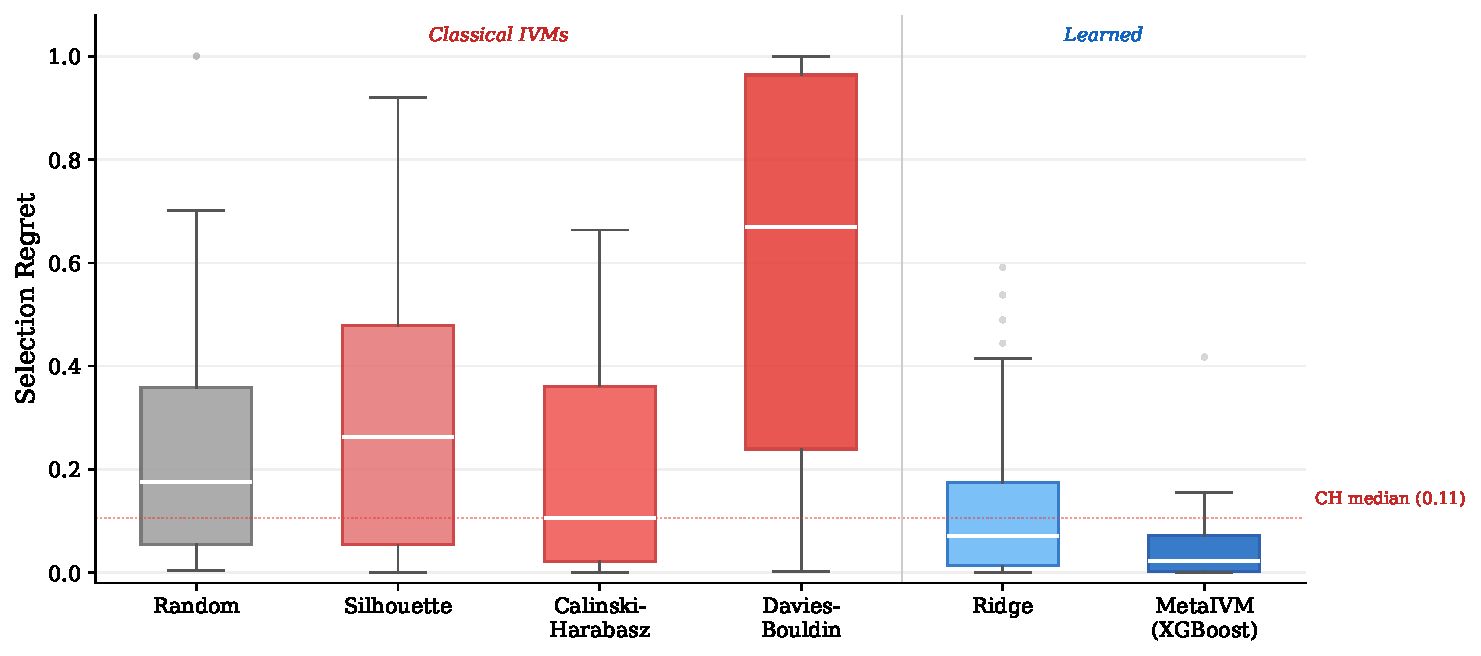
\includegraphics[width=\textwidth]{figure1_regret_boxplot.pdf}
\caption{Distribution of selection regret over the 230 seed--dataset test evaluations (5-seed 60/20/20 dataset-level split protocol; 46 test datasets per seed; 158 unique datasets appearing in at least one test fold), using the default 28-feature set (partition statistics + partition-data interaction + graph; no dataset descriptors, IVM, or algorithm features). \ours{} (XGBoost) has the lowest median regret and fewest catastrophic failures. Classical IVMs show high variance with frequent regret $> 0.5$.}
\label{fig:regret}
\end{figure}

A critical observation: even simple linear regression (Ridge) with our features achieves 0.088 regret, already outperforming all classical IVMs (strongest classical baseline: CH at 0.217; density-based DBCV at 0.219 on the same folds) by a wide margin. This shows that the gains are primarily driven by the meta-learning formulation and feature design. XGBoost provides a further 19\% relative improvement over Ridge (0.071 vs.\ 0.088, $p = 0.022$ by paired Wilcoxon, Table~\ref{tab:significance}) by learning nonlinear feature interactions, but the linear model alone suffices to demonstrate the advantage of our approach over all IVM baselines.

\paragraph{Performance by dataset source.} Because our benchmark is synthetic-heavy (123/223 datasets), a natural concern is whether the aggregate result is driven by synthetic data. Table~\ref{tab:by_source} reports performance stratified by dataset source, pooled across the 230 seed--dataset test evaluations. \ours{} outperforms classical IVMs on every slice: on real-only data (regret 0.076 vs.\ CH 0.226) and on synthetic-only data (0.068 vs.\ CH 0.210) the improvements are similar in magnitude, and analogous patterns hold for OpenML, text, and image subsets individually. The aggregate result is not driven by synthetic data alone.

\begin{table}[t]
\centering
\caption{Performance stratified by dataset source. $N$ is the total number of (seed, dataset) test evaluations pooled across the 5-seed 60/20/20 protocol; the totals sum to 230 across all slices. Learned models use the default 28-feature \ours{} configuration. Regret is the mean over pooled evaluations, matching the source-stratified rows in Table~\ref{tab:shifts} exactly. \ours{} outperforms classical IVMs on every slice; real-data performance is comparable to synthetic.}
\label{tab:by_source}
\small
\begin{tabular}{lrccc}
\toprule
\textbf{Slice} & $N$ & \textbf{\ours{} regret} $\downarrow$ & \textbf{CH regret} & \textbf{Silhouette regret} \\
\midrule
All & 230 & $\mathbf{.071}$ & $.217$ & $.342$ \\
\midrule
Synthetic only & 122 & $\mathbf{.068}$ & $.210$ & $.406$ \\
Real only (OpenML+text+image) & 108 & $\mathbf{.076}$ & $.226$ & $.286$ \\
\midrule
\hspace{1em}OpenML only & 100 & $\mathbf{.079}$ & $.207$ & $.270$ \\
\hspace{1em}Text only & 5 & $\mathbf{.063}$ & $.223$ & $.250$ \\
\hspace{1em}Image only & 3 & $\mathbf{.021}$ & $.563$ & $.594$ \\
\bottomrule
\end{tabular}
\end{table}

\subsection{Isolating the Source of Improvement}

To determine whether the gain comes from \emph{learning per se}, the \emph{per-partition formulation}, or the \emph{feature space}, we compare against three principled learned baselines (Table~\ref{tab:baselines}).

\begin{table}[t]
\centering
\caption{Learned baselines isolating the source of improvement (5 seeds). Learning alone (B1) does not help; dataset-level meta-selection (B3) improves over CH but remains far from per-partition scoring; partition-level features are essential.}
\label{tab:baselines}
\small
\begin{tabular}{lrcc}
\toprule
\textbf{Method} & $d$ & \textbf{Regret} $\downarrow$ & \textbf{Spearman} $\rho$ $\uparrow$ \\
\midrule
\multicolumn{4}{l}{\textit{Fixed IVMs (no learning)}} \\
Raw Silhouette & -- & $.342$ & $.433$ \\
Raw Calinski-Harabasz & -- & $.217$ & $.604$ \\
\midrule
\multicolumn{4}{l}{\textit{Learned baselines: prior work reproduced on our benchmark}$^\ddagger$} \\
AutoClust-style~\citep{poulakis2020autoclust} & 4 & $.195 \pm .028$ & -- \\
PoAC-style~\citep{dasilva2024poac} & 117 & $.139 \pm .025$ & -- \\
\midrule
\multicolumn{4}{l}{\textit{Learned baselines: controls isolating the source of improvement}} \\
B1: Ridge on 3 IVMs (AutoClust-simplified) & 3 & $.337$ & $.391$ \\
B2: XGB on IVM + dataset desc. (PoAC-simplified) & 17 & $.143$ & $.666$ \\
B3: Dataset-level meta-selector$^\dagger$ & 14 & $.180$ & -- \\
\midrule
\multicolumn{4}{l}{\textit{\ours{} (per-partition features)}} \\
Ridge (\texttt{partition\_x\_graph}, 28 features, no IVM) & 28 & $.088$ & $.662$ \\
\textbf{\ours{} XGB (\texttt{partition\_x\_graph}, 28 feat, no IVM)} & \textbf{28} & $\mathbf{.071}$ & $\mathbf{.748}$ \\
\bottomrule
\multicolumn{4}{l}{\footnotesize $^\dagger$Best of 5-NN, Ridge, and XGBoost on same descriptors (Ridge selected).} \\
\multicolumn{4}{l}{\footnotesize $^\ddagger$Both are our reproductions (no public code released with either paper); see Appendix~\ref{app:baseline_reproductions} for details.}
\end{tabular}
\end{table}

These baselines are designed as controls to isolate the source of improvement, not as exhaustive alternatives. Four findings emerge:
\begin{enumerate}
    \item \textbf{Learning IVMs alone does not help} (B1: regret 0.337 $\approx$ raw Silhouette). The three classical IVM scores do not contain enough complementary signal for a learned combination to meaningfully improve selection.
    \item \textbf{Dataset-level meta-selection helps but is insufficient} (B3: 0.180 vs.\ strongest classical baseline CH 0.217). The best dataset-level meta-selector (Ridge on 14 dataset descriptors, selected from 5-NN/Ridge/XGBoost via validation) improves over every classical IVM, showing that dataset-level learning is useful. However, it remains far worse than per-partition \ours{} (0.071), indicating that dataset-level descriptors alone are insufficient and that observing the candidate partition is critical.
    \item \textbf{Adding dataset context helps but plateaus} (B2: 0.143). IVM scores combined with dataset descriptors improve over raw IVMs, but without partition-level features the model cannot distinguish between different clusterings of the same dataset.
    \item \textbf{Prior learned-surrogate methods reproduced on our benchmark} confirm the same pattern. AutoClust-style (MLP on classical CVIs of the candidate) achieves regret $0.195 \pm 0.028$, a modest improvement over the best single classical IVM (CH, 0.217): learned regression over a handful of CVIs helps only marginally. PoAC-style (Random Forest on 115 PyMFE columns + 2 CVIs; 117 features total) does better at $0.139 \pm 0.025$, showing that dataset-level meta-features contribute additional signal, but still substantially worse than per-partition \ours{} (0.071). The progression $\text{CH } 0.217 \to \text{AutoClust-style } 0.195 \to \text{PoAC-style } 0.139 \to \ours{}\ 0.071$ is consistent with a substantial contribution from partition-structural features (supported more directly by the matched B1/B2 controls and feature ablations); PoAC and \ours{} also differ in model class and reproduction protocol, so this progression is corroborating rather than causally isolating.
\end{enumerate}

\paragraph{Where does the improvement come from?} The aggregate gains above are concentrated on datasets where classical IVMs fail. Stratifying test datasets by CH difficulty:

\begin{table}[t]
\centering
\caption{Conditional performance by CH difficulty on a single representative test fold (seed 0, $N = 46$ datasets, default 28-feature XGBoost). Stratification is by per-dataset CH regret computed on that fold. This table is an illustrative slice of the aggregate result in Table~\ref{tab:main}, not a re-aggregation across all 230 seed-dataset pairs; the numerical values are single-seed and should be read as showing \emph{where} the improvement is concentrated rather than as full-benchmark uncertainty estimates. \ours{} provides the largest gains on hard datasets (CH regret $> 0.3$), winning 13 out of 14 cases.}
\label{tab:conditional}
\small
\begin{tabular}{lrccc}
\toprule
\textbf{Regime} & $N$ & \textbf{CH regret} & \textbf{\ours{} regret} & \textbf{Gain} \\
\midrule
Easy (CH $\leq$ 0.05) & 19 & $.015$ & $.050$ & $-.035$ \\
Medium ($0.05 <$ CH $\leq 0.3$) & 13 & $.114$ & $.057$ & $+.058$ \\
Hard (CH $> 0.3$) & 14 & $.514$ & $.142$ & $+.372$ \\
\midrule
All & 46 & $.195$ & $.080$ & $+.115$ \\
\bottomrule
\end{tabular}
\end{table}

On \textbf{easy datasets} where CH already succeeds (regret $\leq 0.05$), \ours{} is slightly worse; it over-refines simple cases where the best partition is obvious. On \textbf{hard datasets} where CH fails badly (regret $> 0.3$), \ours{} reduces regret from 0.514 to 0.142, a 72\% improvement, winning 13 out of 14 cases. This is where the method's value is concentrated: precisely the datasets where classical IVMs provide no useful guidance. A natural follow-up question is whether a hybrid strategy (trusting CH when it is reliable and \ours{} otherwise) could combine their strengths. The challenge is that identifying CH's reliability regime \emph{without labels} is itself the core problem; \ours{} is learning exactly that decision boundary from observable partition and dataset statistics.

\subsection{Candidate-Pool Robustness}
\label{sec:pool_robust}

Since regret is defined relative to the candidate pool, a natural concern is whether \ours{} is specialized to the specific menu of algorithms tested. To assess this, we train \ours{} on the full pool and evaluate on systematically modified pools at test time. \ours{} outperforms CH across \emph{all 11 pool configurations tested}, including: dropping each individual algorithm family (regret 0.048--0.059 vs.\ CH 0.134--0.205), restricting to KMeans-only candidates (0.036 vs.\ 0.085), restricting to density-based candidates only (0.023 vs.\ 0.119), random 50\% subsampling per dataset (0.055 vs.\ 0.174), and filtering by cluster count $k \leq 3$ or $k \geq 5$ (0.042--0.054 vs.\ 0.127--0.139). Notably, the model trained on the full pool generalizes to pools that contain only a single algorithm family at test time. The full breakdown is in Table~\ref{tab:pool_robust} (Appendix). This supports the view that the learned surrogate captures a general ranking principle over partition quality, not a pool-specific selection rule.

\subsection{Feature Ablation (Experiment 2)}

Table~\ref{tab:ablation} shows the impact of different feature groups. The key findings are:

\begin{table}[t]
\centering
\caption{Feature ablation (XGBoost, 5 seeds). $d$ = number of features. ``All features'' includes IVM + algorithm encoding (56 total). Differences from Table~\ref{tab:main} reflect different feature sets.}
\label{tab:ablation}
\small
\begin{tabular}{lrcc}
\toprule
\textbf{Feature Set} & $d$ & \textbf{Regret} $\downarrow$ & \textbf{Spearman} $\rho$ $\uparrow$ \\
\midrule
Dataset descriptors only & 14 & $.303$ & -- \\
IVM only & 3 & $.188$ & $.614$ \\
Graph only & 6 & $.096$ & $.700$ \\
Partition only$^*$ & 22 & $.082$ & $.747$ \\
\midrule
Partition + dataset & 36 & $.078$ & $.746$ \\
\textbf{No IVM, no algorithm} & \textbf{42} & $\mathbf{.068}$ & $\mathbf{.777}$ \\
\midrule
No IVM features & 53 & $.067$ & $.757$ \\
No algorithm features & 45 & $.071$ & $.745$ \\
All features & 56 & $.071$ & $.742$ \\
\midrule
Compact: top-15 features & 15 & $.092$ & $.749$ \\
Compact: top-8 features & 8 & $.094$ & $.737$ \\
\bottomrule
\multicolumn{4}{l}{\footnotesize $^*$Includes partition statistics (12) + partition-data interaction features (10).}
\end{tabular}
\end{table}

\begin{enumerate}
    \item \textbf{IVMs as features are useful but not necessary}: Removing all 3 IVM features barely affects performance (regret 0.067 without IVM vs.\ 0.071 with all 56 features). The model without any IVM or algorithm input (42 features, regret 0.068) still dramatically outperforms all classical IVMs (strongest classical baseline: CH at 0.217). This directly addresses the concern that \ours{} is ``just a learned correction layer on top of CH.''
    \item \textbf{Partition statistics alone are powerful} (regret 0.074, 22 features), outperforming all classical IVMs. Simple features like cluster entropy, Gini impurity, and size ratios carry substantial signal.
    \item \textbf{Graph features alone} (6 features, regret 0.100) already outperform all IVMs, because $k$NN graph conductance captures cluster separability robustly across shapes.
    \item \textbf{A compact 15-feature model} (selected as the 15 most important features, stable across $\geq$3 of 5 training seeds) achieves 0.092 regret, still far better than any IVM. Eight features stable across \emph{all} seeds achieve 0.094 regret.
\end{enumerate}

\subsection{Robustness to Algorithm Diversity (Experiment 3)}

To test whether the model depends on seeing all algorithm families during training, we perform leave-one-algorithm-out evaluation (Table~\ref{tab:loo} in Appendix). Removing DBSCAN has the largest impact ($\Delta = +0.023$ regret), consistent with its unique ability to discover non-convex clusters. All other algorithms have minimal impact ($\Delta < 0.007$), indicating robust generalization.

\paragraph{Leave-one-generator-family-out.} Random 60/20/20 splits may overestimate cross-family transfer because synthetic datasets from closely-related generators appear in both train and test folds. To probe this we hold out entire synthetic generator families and retrain \ours{} on the remaining 211-220 datasets. Across the 12 synthetic families with at least 3 datasets, mean regret is $0.145$ (vs.\ $0.071$ under random CV), maximum $0.487$. Most families transfer well: \texttt{grid} $0.025$, \texttt{aniso} $0.026$, \texttt{ellipsoidal} $0.049$, \texttt{elongated} $0.050$, \texttt{circles} $0.056$, \texttt{noisy} $0.059$, \texttt{varying} $0.075$, \texttt{spirals} $0.093$, \texttt{blobs} $0.094$. Three families degrade substantially: \texttt{moons} $0.358$ (only 4 datasets; no manifold-arc analog remains), \texttt{subspace} $0.375$ (specific structural pattern), \texttt{imb} $0.487$ (holding out all imbalanced datasets removes the training signal for imbalance-adaptive scoring). The pattern is consistent with our operative assumption A1 (Section~\ref{sec:assumptions}): transfer succeeds when the held-out family shares $\phi$-space with the remaining training pool and degrades when it does not. Full breakdown in Appendix (\texttt{logfo\_results.csv}).

\subsection{Cross-Domain Transfer (Experiment 6)}

We frame these experiments as a diagnostic for the distributional-support assumption (A1) introduced in Section~\ref{sec:assumptions}. Can a model trained on one type of dataset generalize to another? Training exclusively on synthetic point-cloud datasets (blobs, ellipsoids, manifolds) and testing on real-world tabular data yields 0.100 regret vs.\ CH's 0.235, with $\rho = 0.887$ on unseen image and text datasets (vs.\ CH's 0.722). Transfer is asymmetric: real$\to$synthetic is weaker (0.238) and underperforms raw CH on synthetic targets (0.193), suggesting synthetic data provides broader $\phi$-space coverage. Read through the lens of (A1), the 0.071 (in-distribution) vs.\ 0.100 (mild shift) vs.\ 0.238 (severe shift) progression quantifies the cost of moving outside the training feature support. Full breakdown in Table~\ref{tab:transfer} (Appendix).

\subsection{Additional Analyses}

On the representative seed-0 test fold, the predicted-versus-true AMI scatter (Figure~\ref{fig:scatter}, Appendix) shows strong agreement ($R^2 = 0.810$; the figure visualizes a single fold and full 5-seed aggregates are in Table~\ref{tab:correlation}). Over the full 230 seed--dataset test evaluations, \ours{} achieves per-dataset Spearman $\rho = 0.748 \pm 0.259$, compared to $\rho = 0.604 \pm 0.320$ for CH (the strongest of the three standard compactness-separation IVMs by $\rho$; Table~\ref{tab:correlation}, Appendix). When all 56 features are used, Calinski-Harabasz is the top feature (35\% importance), yet removing it barely hurts (Table~\ref{tab:ablation}): the model appears to route around CH via redundant structural features when CH is misleading. A compact 15-feature model achieves 0.092 regret, still far better than any IVM. Per-category analysis (Table~\ref{tab:adaptive}) shows that \ours{} adapts its reliance across geometries: variance heterogeneity dominates on ellipsoidal clusters (81\%), conductance on manifolds (20\%), cluster size statistics on imbalanced data (60\%). This adaptive behavior, which no fixed IVM can exhibit, is consistent with the observed performance gap.

\paragraph{Controlled shifts along dataset properties.} To characterize where the improvement is uniform vs.\ concentrated, we bin the 5-seed per-dataset regrets along five axes: number of classes $k$, feature dimensionality $d$, dataset size $n$, class imbalance ratio, and source (Table~\ref{tab:shifts}). Mean regret is essentially flat across $k \in [2, 21+]$ (range $0.039$--$0.083$) and across imbalance regimes ($0.035$--$0.099$). Dimensionality shows a mild trend: $d \in [6, 15]$ is best at $0.047$, $d > 50$ worst at $0.104$. Dataset size shows a similar mild trend: $n < 3000$ averages $0.070$, $n > 3000$ averages $0.093$. OpenML and synthetic sources achieve comparable regrets on pooled held-out evaluations ($0.079$ vs.\ $0.068$), with real overall (OpenML + text + image, $N = 108$) at $0.076$; the aggregate result is not synthetic-driven.

\begin{table}[t]
\centering
\caption{Controlled shifts: \ours{} regret across 5-seed per-dataset evaluations, binned by dataset property. $N$ counts (seed, dataset) pairs in each bin. Regret is roughly flat across $k$ and imbalance; mild dependence on $d$ and $n$ at the extremes; real data (OpenML) is comparable to synthetic.}
\label{tab:shifts}
\small
\begin{tabular}{llrl}
\toprule
\textbf{Axis} & \textbf{Bin} & $N$ & \textbf{Regret (mean $\pm$ std)} \\
\midrule
\multirow{5}{*}{$n_{\text{classes}}$}
  & $k = 2$ & 58 & $.083 \pm .119$ \\
  & $k \in [3, 5]$ & 85 & $.081 \pm .122$ \\
  & $k \in [6, 10]$ & 69 & $.059 \pm .072$ \\
  & $k \in [11, 20]$ & 14 & $.039 \pm .076$ \\
  & $k \geq 21$ & 4 & $.063 \pm .089$ \\
\midrule
\multirow{4}{*}{Dimensionality}
  & $d \leq 5$ & 90 & $.083 \pm .129$ \\
  & $d \in [6, 15]$ & 48 & $.047 \pm .064$ \\
  & $d \in [16, 50]$ & 72 & $.066 \pm .081$ \\
  & $d > 50$ & 20 & $.104 \pm .135$ \\
\midrule
\multirow{3}{*}{Dataset size $n$}
  & $500 \leq n < 1500$ & 117 & $.070 \pm .114$ \\
  & $1500 \leq n < 3000$ & 64 & $.060 \pm .088$ \\
  & $n > 3000$ & 49 & $.093 \pm .103$ \\
\midrule
\multirow{4}{*}{Imbalance ratio}
  & Balanced ($<1.5$) & 158 & $.071 \pm .113$ \\
  & Mild ($1.5$--$3$) & 24 & $.086 \pm .073$ \\
  & Moderate ($3$--$10$) & 24 & $.035 \pm .025$ \\
  & Extreme ($>10$) & 24 & $.099 \pm .125$ \\
\midrule
\multirow{4}{*}{Source}
  & Synthetic & 122 & $.068 \pm .120$ \\
  & OpenML & 100 & $.079 \pm .088$ \\
  & Text & 5 & $.063 \pm .082$ \\
  & Image & 3 & $.021 \pm .029$ \\
\bottomrule
\end{tabular}
\end{table}

\begin{table}[t]
\centering
\caption{Dominant features shift across dataset geometries; the model adapts its reliance to data structure.}
\label{tab:adaptive}
\small
\begin{tabular}{llp{5.5cm}}
\toprule
\textbf{Dataset type} & \textbf{Dominant feature (importance)} & \textbf{Why it matters} \\
\midrule
Spherical clusters & Entropy (0.54) & Balanced cluster sizes signal correct $k$ \\
Ellipsoidal clusters & Within-var std (0.81) & Heterogeneous variance reveals shape mismatch \\
Manifold clusters & Conductance (0.20) & Graph structure captures non-convex geometry \\
Imbalanced clusters & Cluster size std (0.60) & Correct partitions preserve the imbalance pattern \\
Real-world data & Entropy (0.17), centroid sep (0.11) & No single signal dominates \\
\bottomrule
\end{tabular}
\end{table}

The improvement over Silhouette, Calinski-Harabasz, and Davies-Bouldin is highly significant (paired Wilcoxon $p < 10^{-12}$; Table~\ref{tab:significance}, Appendix). We do not report a $p$-value against DBCV or S\_Dbw because these were added post-hoc after the Wilcoxon analysis was run. The method is robust across four external metrics: AMI, ARI, NMI, and V-measure all show consistent rankings (Table~\ref{tab:multitarget}, Appendix). With just 13 training datasets (10\%), \ours{} already achieves 0.116 regret, better than all IVMs (Table~\ref{tab:learning}, Appendix). Zero-engineering approaches (graph spectral embeddings, GNN) also outperform all IVMs (Appendix~\ref{app:zero_engineering}), suggesting the formulation is robust to feature design choices.

Failure analysis (Table~\ref{tab:failure}, Appendix) reveals that the model struggles on datasets with high noise, subspace structure, or extreme imbalance; 19\% of test datasets have regret $> 0.15$. Text and image domains have zero high-regret cases.


\subsection{Extension: Graph Community Detection}
\label{sec:graph_community}

Classical IVMs require point coordinates and \textbf{cannot be applied} to graph community detection. \ours{} is naturally applicable because our graph-only features (conductance, edge density, normalized cut proxy) require only the adjacency structure and a partition. We evaluate on 80 benchmark graphs (SBM, 2--10 communities, 5 algorithms at multiple resolutions; Table~\ref{tab:graph_community}).

\begin{table}[t]
\centering
\caption{Community detection model selection on 80 benchmark graphs (2,000 runs, 5 seeds). Classical IVMs (Silhouette, CH, DB) cannot be computed because no point coordinates exist. \ours{} outperforms all graph-based heuristics.}
\label{tab:graph_community}
\small
\begin{tabular}{lcc}
\toprule
\textbf{Method} & \textbf{Regret} $\downarrow$ & \textbf{Spearman} $\rho$ $\uparrow$ \\
\midrule
\multicolumn{3}{l}{\textit{Not applicable (require point coordinates)}} \\
Silhouette / CH / DB & n/a & n/a \\
\midrule
\multicolumn{3}{l}{\textit{Graph-based heuristics}} \\
Random & $.259 \pm .318$ & -- \\
Edge-cut fraction$^\ast$ & $.677 \pm .341$ & $-.259 \pm .489$ \\
Conductance & $.655 \pm .357$ & $-.226 \pm .506$ \\
Modularity & $.045 \pm .088$ & $.872 \pm .205$ \\
\midrule
\textbf{\ours{} (graph features)} & $\mathbf{.018 \pm .044}$ & $\mathbf{.946 \pm .107}$ \\
\bottomrule
\multicolumn{3}{l}{\footnotesize Regret uses NMI as the external agreement metric (no point coordinates, so AMI's} \\
\multicolumn{3}{l}{\footnotesize permutation model is unavailable for some graph baselines). $^\ast$The edge-cut fraction} \\
\multicolumn{3}{l}{\footnotesize (between-cluster edges / total edges) coincides with $1-$coverage; as a selection rule it is} \\
\multicolumn{3}{l}{\footnotesize identical to a coverage-maximizing selector, so we report the two as a single baseline.} \\
\end{tabular}
\end{table}

\ours{} achieves 0.018 regret ($\rho = 0.946$), a 61\% reduction over modularity, while the edge-cut fraction and conductance are both anti-correlated with external agreement ($\rho < 0$). On a preliminary set of 7 real-world attributed graphs (Table~\ref{tab:attr_graph}, Appendix), a leave-one-graph-out evaluation places \ours{} below modularity (0.004 vs.\ 0.028 regret); with only 7 graphs this is a high-variance, preliminary indication rather than a headline result. Together, these experiments suggest that the surrogate-learning principle extends to settings where classical IVMs cannot operate.


%% ============================================================
\section{Discussion}
\label{sec:discussion}
%% ============================================================

\paragraph{Why do IVMs fail, and why does \ours{} succeed?} Classical IVMs measure fixed geometric properties that correlate with external agreement only when clusters match geometric assumptions. Our analysis (Table~\ref{tab:adaptive}) reveals that the predictive signal shifts across regimes, and no fixed IVM can adapt. Ablations support that gains come from the formulation and feature space: Ridge alone beats all IVMs, removing IVM features barely hurts, and learned baselines (Table~\ref{tab:baselines}) show neither learning alone nor dataset-level selection suffice. The model uses CH when informative and routes around it when misleading.

\paragraph{Scope and assumptions.} Our goal is not universal clustering quality but a surrogate for external agreement in settings where benchmark labels define the reference partition offline. This is a supervised surrogate-learning setup for unsupervised deployment (not circular, but bounded): the method inherits the notion of quality used in training. Multi-target analysis (Table~\ref{tab:multitarget}, Appendix) shows robustness across AMI, ARI, NMI, and V-measure, but we do not claim robustness to arbitrary task-specific criteria. Pointwise regression and ranking losses achieve similar regret (Table~\ref{tab:ranking_objectives}, Appendix), suggesting the formulation matters more than the loss.

\paragraph{When are classification labels an appropriate clustering target?} Our benchmarks treat each dataset's classification labels as the reference partition for AMI. This is an operational choice: classification labels provide an unambiguous, reproducible ground truth and are the same target used by most prior meta-learning work on clustering. In some real-world applications, however, the ``natural'' clustering may differ from the labeled classification: customers can be grouped by demographics, purchase behavior, lifetime value, or risk profile, all valid, all producing different partitions. \ours{} is a framework, not a specific policy about what counts as a good clustering: the same infrastructure would work with hierarchical labels, application-specific tags, or user-defined similarity signals, provided a labeled meta-benchmark exists. Users deploying \ours{} with a specific application clustering goal in mind should retrain on labeled examples that reflect that goal; where the deployment target matches the benchmark target (classification-label recovery on tabular / image / text data), our results are directly applicable. This limitation is inherent to any supervised surrogate for unsupervised evaluation and is shared with AutoClust~\citep{poulakis2020autoclust}, PoAC~\citep{dasilva2024poac}, and dataset-level meta-selection work.

\paragraph{Label semantics.} We do not claim that benchmark class labels define the uniquely correct clustering of a dataset. \ours{} learns to predict agreement with the reference partitions used in training. This is appropriate when users want clusters aligned with semantic labels similar to those in the training benchmark (e.g., disease subtypes, object classes, curated taxonomies). It is less appropriate when the desired clustering is task-specific, multi-resolution, or orthogonal to class labels. In such cases, the relevant notion of quality must be encoded in the training distribution.

\paragraph{Benchmark dependence and generalization.} Our benchmark is synthetic-heavy (123/223 datasets) by design for controlled geometry coverage, not as a natural-frequency sample. The transfer asymmetry (synthetic$\to$real: 0.100, real$\to$synthetic: 0.238) confirms distribution dependence. On pooled held-out OpenML evaluations, \ours{} achieves 0.079 regret vs.\ CH's 0.207 (Table~\ref{tab:by_source}); on 8 hard real datasets (CH regret $> 0.3$), \ours{} wins all 8. The graph extension provides evidence beyond Euclidean data. Limited non-tabular evidence (5 text, 4 image) tempers cross-modality claims. Deployment cost is negligible: $< 1$\,s feature extraction, $< 0.2$\,ms inference, cheaper than Silhouette (Table~\ref{tab:complexity}, Appendix).

\paragraph{Limitations.} (1) Requires offline training on labeled datasets (mitigated: can use purely synthetic data). (2) Predicts external agreement (AMI), one operationalization of quality; domain-specific criteria may differ. (3) Limited evidence on specialized domains (genomics, time series). (4) Main benchmark omits Spectral Clustering ($O(n^3)$); post-hoc inclusion increases regret by only 0.005. (5) Struggles on high-noise, subspace, and extreme-imbalance datasets (19\% of test cases above regret 0.15). (6) The AutoClust-style baseline is a partial reproduction using four of the ten original CVIs; the other six (SDbw, CDBw, Tau, Ratkowsky-Lance, McClain-Rao, C-Index) lack maintained Python implementations. The effect of the unavailable six CVIs on the reproduction regret remains unknown.


%% ============================================================
\section{Conclusion}
\label{sec:conclusion}
%% ============================================================

On our benchmark, external-agreement-based clustering model selection is substantially better served by a learned surrogate than by any fixed IVM. \ours{} reduces selection regret by 67\% over the strongest classical baseline (Calinski-Harabasz, 0.217), with the improvement over Silhouette, CH, and DB significant at Wilcoxon $p < 10^{-12}$; density-based measures added in this revision (DBCV 0.219, S\_Dbw 0.334) are comparable to but no better than CH on the same protocol. Improvements are robust across metrics and models and extend to graph community detection. Principled controls confirm that the gains come from the per-partition formulation and feature space, not from learning alone or the inclusion of IVMs. Performance depends on the training distribution, and generalization to domains far from our benchmark remains an open question. We will release all data, code, and pre-trained models.

\paragraph{Ethics and reproducibility.}
We foresee no significant negative societal impact. The benchmark uses only publicly available datasets. All code, datasets, pre-trained models, and experiment scripts will be released as open-source. The benchmark is fully reproducible with fixed random seeds (0--4) for all splits.


%% ============================================================
% References
%% ============================================================
\bibliography{references}
\bibliographystyle{tmlr}


%% ============================================================
% APPENDIX
%% ============================================================
\appendix

\section{Complete Feature Descriptions}
\label{app:features}

Table~\ref{tab:app_features} lists all 56 features extracted for each (dataset, partition) pair, grouped by source.

\begin{table}[h]
\centering
\caption{Complete feature list. All features are computed without access to ground-truth labels.}
\label{tab:app_features}
\small
\begin{tabular}{lp{7cm}}
\toprule
\textbf{Feature} & \textbf{Description} \\
\midrule
\multicolumn{2}{l}{\textit{Partition statistics (12 features)}} \\
\texttt{n\_clusters} & Number of clusters in the partition \\
\texttt{noise\_fraction} & Fraction of points assigned to noise ($-1$ label) \\
\texttt{cluster\_size\_\{min,max,mean,std,median\}} & Statistics of cluster sizes \\
\texttt{size\_ratio} & Ratio of largest to smallest cluster \\
\texttt{entropy} & Shannon entropy of the cluster size distribution \\
\texttt{gini} & Gini impurity of cluster assignments \\
\texttt{imbalance} & Deviation from uniform cluster sizes \\
\texttt{singleton\_fraction} & Fraction of clusters with a single point \\
\midrule
\multicolumn{2}{l}{\textit{Dataset descriptors (14 features)}} \\
\texttt{ds\_n\_samples}, \texttt{ds\_n\_features} & Dataset dimensions \\
\texttt{ds\_log\_n}, \texttt{ds\_log\_d} & Log-transformed dimensions \\
\texttt{ds\_d\_over\_n} & Dimensionality ratio $d/n$ \\
\texttt{ds\_mean\_of\_\{means,stds,skewness,kurtosis\}} & Feature-wise distribution statistics (averaged) \\
\texttt{ds\_sparsity} & Fraction of near-zero entries \\
\texttt{ds\_intrinsic\_dim\_pca95} & PCA components for 95\% variance \\
\texttt{ds\_pairwise\_dist\_\{mean,std,median\}} & Pairwise distance statistics (subsampled to 2k points) \\
\midrule
\multicolumn{2}{l}{\textit{Partition-data interaction features (10 features)}} \\
\texttt{within\_cluster\_var\_\{mean,std\}} & Within-cluster variance statistics \\
\texttt{between\_cluster\_var} & Between-cluster variance \\
\texttt{dispersion\_ratio} & Between / within variance ratio \\
\texttt{cluster\_density\_\{mean,std,max\}} & Average pairwise distance within clusters \\
\texttt{centroid\_sep\_\{min,mean,std\}} & Pairwise centroid distance statistics \\
\midrule
\multicolumn{2}{l}{\textit{Graph-based features (6 features)}} \\
\texttt{graph\_cut\_fraction} & Fraction of $k$NN edges crossing cluster boundaries \\
\texttt{graph\_normalized\_cut\_proxy} & Proxy for the normalized graph cut \\
\texttt{graph\_within\_cluster\_edge\_density} & Mean edge density within clusters \\
\texttt{graph\_within\_edge\_density\_std} & Std of within-cluster edge density \\
\texttt{graph\_conductance\_\{min,mean\}} & Graph conductance statistics \\
\midrule
\multicolumn{2}{l}{\textit{IVM features (3 features)}} \\
\texttt{ivm\_silhouette} & Silhouette Coefficient \\
\texttt{ivm\_calinski\_harabasz} & Calinski-Harabasz Index \\
\texttt{ivm\_davies\_bouldin\_neg} & Negated Davies-Bouldin Index \\
\midrule
\multicolumn{2}{l}{\textit{Algorithm encoding (11 features)}} \\
\texttt{algo\_\{KMeans,...,Agglom.\}} & One-hot encoding of algorithm family (6) \\
\texttt{hp\_\{n\_clusters,...,min\_cluster\_size\}} & Numeric hyperparameter values (5) \\
\bottomrule
\end{tabular}
\end{table}


\section{Feature Importance}
\label{app:importance}

Table~\ref{tab:app_importance} shows the complete XGBoost feature importance ranking. The top 5 features account for 62\% of total importance; the top 15 account for 84\%.

\begin{table}[h]
\centering
\caption{Complete feature importance ranking (XGBoost gain). Features below 0.5\% omitted for brevity.}
\label{tab:app_importance}
\small
\begin{tabular}{rlr}
\toprule
\textbf{Rank} & \textbf{Feature} & \textbf{Importance} \\
\midrule
1 & \texttt{ivm\_calinski\_harabasz} & 34.96\% \\
2 & \texttt{ds\_mean\_of\_kurtosis} & 9.75\% \\
3 & \texttt{graph\_conductance\_min} & 7.96\% \\
4 & \texttt{cluster\_size\_mean} & 4.64\% \\
5 & \texttt{ds\_sparsity} & 4.43\% \\
6 & \texttt{entropy} & 4.31\% \\
7 & \texttt{ds\_pairwise\_dist\_std} & 4.08\% \\
8 & \texttt{ds\_mean\_of\_skewness} & 2.57\% \\
9 & \texttt{ds\_d\_over\_n} & 2.15\% \\
10 & \texttt{between\_cluster\_var} & 1.81\% \\
11 & \texttt{noise\_fraction} & 1.72\% \\
12 & \texttt{ds\_n\_features} & 1.62\% \\
13 & \texttt{gini} & 1.61\% \\
14 & \texttt{ivm\_silhouette} & 1.59\% \\
15 & \texttt{ds\_n\_samples} & 1.48\% \\
16 & \texttt{singleton\_fraction} & 1.43\% \\
17 & \texttt{cluster\_density\_mean} & 1.18\% \\
18 & \texttt{ds\_pairwise\_dist\_median} & 1.08\% \\
19 & \texttt{ds\_mean\_of\_means} & 0.92\% \\
20 & \texttt{algo\_GaussianMixture} & 0.82\% \\
\bottomrule
\end{tabular}
\end{table}

\paragraph{Protocol-specific permutation-importance intervals.} We report permutation importance with a bootstrap uncertainty interval that reflects variability across random permutation realizations at a single split, not variability across datasets or folds. The protocol is: (i) fix the seed-0 split of the 5-seed 60/20/20 dataset-level protocol (train 133 datasets, val 44 datasets, test 46 datasets); (ii) train the default 28-feature XGBoost once on train+val at that split; (iii) for each feature and each of 30 independent random permutations, shuffle that feature's column across the test-fold rows and recompute the selection regret; (iv) construct a 95\% bootstrap interval on the mean $\Delta$ regret across the 30 permutation runs by resampling those 30 realizations 1000 times with replacement (\texttt{numpy.random} with a fixed seed). Table~\ref{tab:app_perm_importance} reports mean $\Delta$ regret and CI endpoints. Features whose lower CI bound remains strictly positive after rounding to four decimals are marked as clearing this protocol-specific threshold; the lower bound for \texttt{graph\_normalized\_cut\_proxy} is $+0.0002$ at four-decimal precision (previously printed as $+0.000$ due to three-decimal rounding). Eight features clear the threshold: \texttt{graph\_conductance\_min}, \texttt{centroid\_sep\_mean}, \texttt{centroid\_sep\_min}, \texttt{noise\_fraction}, \texttt{cluster\_size\_max}, \texttt{cluster\_density\_max}, \texttt{cluster\_size\_std}, and \texttt{graph\_normalized\_cut\_proxy}. Per-feature impacts are modest in absolute magnitude because the 28 features are redundantly informative (removing any single feature still leaves correlated structural features that partially recover the signal). We do not apply a multiple-testing correction, and we do not aggregate the analysis across the other four seeds; the resulting significance statements should be read as protocol-specific rather than as full-benchmark tests of feature relevance.

\begin{table}[h]
\centering
\caption{Permutation importance with 95\% bootstrap CIs (30 permutations, default 28-feature model, seed-0 split of the 5-seed 60/20/20 protocol). $\Delta$ regret is the change in selection regret when the feature is shuffled at test time. Values shown to three decimals except the \texttt{graph\_normalized\_cut\_proxy} row, whose lower bound is $+0.0002$ at four decimals (would round to $+0.000$ otherwise). * = lower 95\% CI strictly $> 0$. Top 20 features shown. See Section~\ref{sec:results} for protocol details and scope caveats.}
\label{tab:app_perm_importance}
\small
\begin{tabular}{lrr}
\toprule
\textbf{Feature} & $\Delta$ \textbf{regret} & \textbf{95\% CI} \\
\midrule
\texttt{graph\_conductance\_min}$^{*}$ & $+0.035$ & $[+0.017, +0.050]$ \\
\texttt{centroid\_sep\_mean}$^{*}$ & $+0.026$ & $[+0.009, +0.043]$ \\
\texttt{centroid\_sep\_min}$^{*}$ & $+0.025$ & $[+0.005, +0.042]$ \\
\texttt{noise\_fraction}$^{*}$ & $+0.022$ & $[+0.014, +0.031]$ \\
\texttt{cluster\_size\_max}$^{*}$ & $+0.020$ & $[+0.010, +0.031]$ \\
\texttt{entropy} & $+0.015$ & $[-0.000, +0.033]$ \\
\texttt{cluster\_density\_max}$^{*}$ & $+0.013$ & $[+0.002, +0.026]$ \\
\texttt{cluster\_size\_std}$^{*}$ & $+0.012$ & $[+0.004, +0.022]$ \\
\texttt{centroid\_sep\_std} & $+0.010$ & $[-0.005, +0.027]$ \\
\texttt{between\_cluster\_var} & $+0.009$ & $[-0.003, +0.023]$ \\
\texttt{within\_cluster\_var\_std} & $+0.009$ & $[-0.001, +0.022]$ \\
\texttt{cluster\_size\_mean} & $+0.009$ & $[-0.005, +0.022]$ \\
\texttt{cluster\_density\_mean} & $+0.009$ & $[-0.001, +0.019]$ \\
\texttt{cluster\_density\_std} & $+0.008$ & $[-0.004, +0.018]$ \\
\texttt{graph\_normalized\_cut\_proxy}$^{*}$ & $+0.008$ & $[+0.0002, +0.0150]$ \\
\texttt{graph\_within\_edge\_density\_std} & $+0.007$ & $[-0.003, +0.016]$ \\
\texttt{cluster\_size\_min} & $+0.006$ & $[-0.005, +0.018]$ \\
\texttt{within\_cluster\_var\_mean} & $+0.006$ & $[-0.005, +0.015]$ \\
\texttt{cluster\_size\_median} & $+0.006$ & $[-0.001, +0.013]$ \\
\texttt{graph\_conductance\_mean} & $+0.005$ & $[-0.005, +0.017]$ \\
\bottomrule
\end{tabular}
\end{table}


\section{Clustering Algorithm Configurations}
\label{app:configs}

Table~\ref{tab:app_configs} details the complete hyperparameter grid for each clustering algorithm (91 configurations in total). At runtime, SpectralClustering was skipped due to $O(n^3)$ complexity, and AgglomerativeClustering was skipped for datasets with $n > 10{,}000$ due to $O(n^2)$ memory. After these filters, the effective count ranges from 19 to 79 per dataset (mean: 75.7; lower counts occur for the largest datasets where additional GMM configurations also fail to converge), yielding 16,889 total runs across 223 datasets.

\begin{table}[h]
\centering
\caption{Clustering algorithm hyperparameter grids. Total configurations: 91 per dataset (before filtering).}
\label{tab:app_configs}
\small
\begin{tabular}{llr}
\toprule
\textbf{Algorithm} & \textbf{Hyperparameters} & \textbf{Configs} \\
\midrule
KMeans & $k \in \{2,3,5,7,10,15,20,30\}$, n\_init $= 10$ & 8 \\
Gaussian Mixture & $k \in \{2,3,5,7,10,15,20\}$, cov $\in \{\text{full},\text{diag}\}$ & 14 \\
Spectral & $k \in \{2,3,5,7,10,15\}$, affinity $\in \{\text{rbf},\text{nn}\}$ & 12$^*$ \\
DBSCAN & $\varepsilon \in \{0.1,0.3,0.5,1.0,2.0,5.0\}$, min\_samp $\in \{3,5,10,20\}$ & 24 \\
HDBSCAN & min\_cluster $\in \{5,10,20,50\}$, min\_samp $\in \{1,5,10\}$ & 12 \\
Agglomerative & $k \in \{2,3,5,7,10,15,20\}$, link $\in \{\text{ward},\text{comp.},\text{avg.}\}$ & 21$^\dagger$ \\
\bottomrule
\multicolumn{3}{l}{\footnotesize $^*$Skipped at runtime (cubic complexity). $^\dagger$Skipped for $n > 10{,}000$ (quadratic memory).}
\end{tabular}
\end{table}


\section{Per-Seed Results}
\label{app:perseeds}

Table~\ref{tab:app_seeds} shows selection regret and Spearman $\rho$ for each method on each of the 5 random seeds. Results are consistent across seeds, with low variance for \ours{}.

\begin{table}[h]
\centering
\caption{Per-seed results for all methods (selection regret / Spearman $\rho$).}
\label{tab:app_seeds}
\small
\begin{tabular}{lccccc}
\toprule
\textbf{Method} & \textbf{Seed 0} & \textbf{Seed 1} & \textbf{Seed 2} & \textbf{Seed 3} & \textbf{Seed 4} \\
\midrule
Random & .170 / .035 & .160 / .030 & .212 / .006 & .171 / .007 & .174 / .019 \\
Global best & .236 / .106 & .159 / .061 & .352 / .024 & .327 / .010 & .130 / .063 \\
Silhouette & .292 / .375 & .390 / .369 & .390 / .478 & .361 / .467 & .276 / .476 \\
Calinski-Harabasz & .195 / .589 & .249 / .573 & .270 / .634 & .230 / .604 & .142 / .621 \\
Davies-Bouldin & .297 / .337 & .393 / .329 & .395 / .427 & .365 / .455 & .277 / .448 \\
CH Adjusted & .229 / .513 & .288 / .490 & .282 / .555 & .282 / .535 & .207 / .559 \\
\midrule
Ridge & .093 / .617 & .111 / .620 & .109 / .710 & .072 / .693 & .055 / .669 \\
MLP & .093 / .614 & .096 / .640 & .096 / .721 & .056 / .734 & .070 / .733 \\
\textbf{\ours{} (XGB)} & \textbf{.080 / .703} & \textbf{.075 / .744} & \textbf{.074 / .808} & \textbf{.060 / .768} & \textbf{.064 / .718} \\
\bottomrule
\end{tabular}
\end{table}


\section{Dataset Collection Details}
\label{app:datasets}

Our benchmark comprises 223 datasets from four sources. Table~\ref{tab:app_stats} provides summary statistics.

\begin{table}[h]
\centering
\caption{Dataset collection summary statistics (across 223 datasets with clustering runs).}
\label{tab:app_stats}
\small
\begin{tabular}{lrrrrr}
\toprule
\textbf{Statistic} & \textbf{Min} & \textbf{Median} & \textbf{Mean} & \textbf{Max} \\
\midrule
Samples ($n$) & 150 & 1,200 & 4,438 & 48,842 \\
Features ($d$) & 2 & 14 & 33 & 500 \\
Classes ($k$) & 2 & 4 & 6.3 & 50 \\
Runs per dataset & 19 & 79 & 75.7 & 91 \\
\bottomrule
\end{tabular}
\end{table}

\paragraph{OpenML datasets (91).}
We selected datasets from the OpenML CC18 benchmark suite~\citep{bischl2016aslib} plus 32 additional hand-selected datasets chosen for domain diversity (biology, finance, physics, social sciences, computer vision). Datasets with $n > 20{,}000$ samples were subsampled uniformly at random; those with $d > 200$ features were reduced to 50 dimensions via PCA. Three datasets (\texttt{openml\_3}, \texttt{openml\_46}, \texttt{openml\_50}) were excluded due to all-NaN features after preprocessing.

\paragraph{Synthetic datasets (123).}
Generated using scikit-learn generators and custom code to systematically vary:
\begin{itemize}
    \item \textbf{Dimensionality}: $d \in \{2, 3, 5, 10, 15, 20, 30, 50, 100, 200\}$
    \item \textbf{Number of clusters}: $k \in \{2, 3, 4, 5, 6, 8, 10, 12, 15, 20\}$
    \item \textbf{Cluster overlap}: Low ($\sigma=0.5$), medium ($\sigma=1.5$), high ($\sigma=3.0$)
    \item \textbf{Cluster shape}: Spherical (blobs), ellipsoidal (random covariance), manifold (Swiss roll, S-curve), non-convex (moons, circles)
    \item \textbf{Imbalance}: Mild (1:1.5:2.5), moderate (1:3:16), extreme (1:1.5:2.5:45), many-small (6 clusters with one dominant)
    \item \textbf{Noise}: 5\%, 15\%, 25\% uniform background noise
    \item \textbf{Subspace structure}: Relevant features in $\{2, 3, 5\}$ out of $\{50, 100, 200\}$ total dimensions
\end{itemize}

\paragraph{Text datasets (5).}
Five subsets of the 20Newsgroups corpus: all categories, science, politics+religion, computers, and recreation. Text was converted to TF-IDF vectors (5,000-word vocabulary, English stop words removed) and reduced to 50 dimensions via truncated SVD. Subsampled to 2,000--5,000 documents.

\paragraph{Image datasets (4).}
MNIST and Fashion-MNIST digit/clothing images, each at 2,000 and 5,000 samples. Pixel features (784 dimensions) were reduced to 50 dimensions via PCA.


\section{Preprocessing Pipeline}
\label{app:preprocessing}

Each dataset undergoes the following preprocessing before clustering:
\begin{enumerate}
    \item \textbf{Missing value handling}: Columns with $>$50\% missing values are dropped. Remaining missing values are imputed with column medians.
    \item \textbf{Constant feature removal}: Features with zero variance are dropped.
    \item \textbf{Standardization}: All features are standardized to zero mean, unit variance.
    \item \textbf{Graph construction}: $k$-nearest-neighbor graphs are computed for $k \in \{10, 15, 20\}$ using Euclidean distance, stored as sparse adjacency matrices.
\end{enumerate}


\section{Zero Feature Engineering Details}
\label{app:zero_engineering}

Table~\ref{tab:zero} compares approaches with varying levels of feature engineering. All results are preliminary (single architectures, no hyperparameter search).

\begin{table}[h]
\centering
\caption{Impact of feature engineering. Even zero-engineering approaches (graph embeddings, GNN) substantially outperform all classical IVMs.}
\label{tab:zero}
\small
\begin{tabular}{llcc}
\toprule
\textbf{Method} & \textbf{Engineering} & \textbf{Regret} $\downarrow$ & \textbf{Spearman} $\rho$ $\uparrow$ \\
\midrule
CH (strongest classical baseline) & n/a & $.217 \pm .237$ & $.604 \pm .320$ \\
DBCV (density-based baseline) & n/a & $.219 \pm .259$ & -- \\
\midrule
XGBoost (graph spectral emb.) & none & $.105 \pm .130$ & $.667 \pm .290$ \\
GNN (end-to-end) & none & $.131 \pm .193$ & $.705 \pm .229$ \\
XGBoost (auto-features, 18) & minimal & $.083 \pm .120$ & $.743 \pm .270$ \\
\textbf{\ours{} (hand-crafted, 56)} & \textbf{heavy} & $\mathbf{.073 \pm .103}$ & $\mathbf{.758 \pm .302}$ \\
\bottomrule
\end{tabular}
\end{table}

The GNN operates directly on the $k$NN graph with partition labels as 32-dimensional one-hot node features (3-layer GIN, 128 hidden dims; see Appendix~\ref{app:training} for details). Despite no feature engineering, it achieves $\rho = 0.705$, above CH ($\rho = 0.604$, the strongest of the three standard IVMs for which ranking metrics were computed). Graph spectral embeddings (top-32 truncated-SVD components of the $k$NN adjacency matrix, mean/std-pooled per cluster and concatenated with partition statistics) fed to XGBoost achieve lower regret (0.105) but lower $\rho$ (0.667). The 18 auto-features (cluster sizes, within/between variance, centroid distances) close most of the gap to the full model. Hand-crafted features provide a further 12\% improvement, primarily through graph conductance and dataset-level descriptors (kurtosis, sparsity).


\section{Model Training Details}
\label{app:training}

\paragraph{XGBoost configuration.}
We use the \texttt{xgboost} Python package with the following hyperparameter search: max depth $\in \{3, 5, 7\}$, learning rate $\in \{0.01, 0.05, 0.1\}$ (9 combinations total). Each configuration is trained with up to 500 estimators and early stopping (patience 20 rounds) on the validation set, using RMSE as the stopping criterion. The best configuration (lowest validation MSE) is then refitted on the combined train+val data using the optimal number of estimators from early stopping. Missing feature values (e.g., IVM scores for degenerate partitions) are handled natively by XGBoost's sparse-aware split finding.

\paragraph{MLP configuration.}
Grid search over hidden layer architectures $\{(256, 128), (512, 256), (256, 128, 64), (512, 256, 128)\}$ and learning rates $\{10^{-3}, 3 \cdot 10^{-3}\}$ (8 configurations total), ReLU activations, Adam optimizer, max 200 iterations. Each configuration is trained on the dataset-level train fold only (not on train + val pooled); scikit-learn's built-in \texttt{early\_stopping} is disabled to avoid within-training-set random splitting that would mix candidate partitions from the same dataset across sklearn's internal train / val. Outer arch/lr model selection uses the dataset-level held-out val fold. Features are standardized to zero mean and unit variance. Missing values are imputed with zeros before scaling. This preserves dataset-level train/val separation throughout all model selection and training decisions.

\paragraph{Ridge regression.}
$L_2$-regularized linear regression with regularization strength $\alpha$ selected from $\{0.01, 0.1, 1.0, 10.0, 100.0\}$ via validation $R^2$ score. The best $\alpha$ is used to refit on the combined train+val data. Features are standardized as above.

\paragraph{GNN configuration.}
3 GIN layers with 128 hidden dimensions, residual connections, batch normalization, 10\% dropout. Partition labels encoded as 32-dimensional one-hot vectors (with hash collision for $k > 31$). Node features truncated/padded to 50 dimensions. Partition-aware pooling: mean within each cluster, then mean across cluster representations, concatenated with global mean pool. Adam optimizer (lr $= 10^{-3}$), batch size 32, max 80 epochs, early stopping patience 15.


\section{Baseline Reproductions: AutoClust-style and PoAC-style}
\label{app:baseline_reproductions}

Neither AutoClust~\citep{poulakis2020autoclust} nor PoAC~\citep{dasilva2024poac} released public code with their paper. We therefore reimplemented each method from the description in the paper. Both reproductions use our 5-seed 60/20/20 dataset-level splits (Section~\ref{sec:setup}) rather than the original evaluation protocols of the source papers, so the reported regret numbers reflect performance on our 223-dataset benchmark rather than on the smaller UCI subsets in the original evaluations. This section documents our reproduction protocol and its deviations from the original descriptions.

\paragraph{AutoClust-style baseline.} The relevant component of AutoClust is the surrogate MLP that maps a candidate partition's classical CVIs to predicted external agreement. From \citet{poulakis2020autoclust} Figure 2 and Table I:
\begin{itemize}
    \item Architecture: hidden layers $60 \to 30 \to 10$, ReLU activations, ADAM optimizer.
    \item Target: external agreement (Adjusted Rand Index; we use AMI here to match the rest of our benchmark. AMI and ARI are strongly correlated on our benchmark, Table~\ref{tab:multitarget}).
    \item Input: a fixed vector of internal CVIs. The original paper uses ten: Silhouette, Dunn, C-Index, Calinski-Harabasz, Davies-Bouldin, SDbw, CDBw, Tau, Ratkowsky-Lance, McClain-Rao.
\end{itemize}
Our reproduction matches the architecture exactly. For the input CVIs, we use four that have maintained Python implementations and that we could compute cleanly for all 16,889 partitions: Silhouette, Calinski-Harabasz, and Davies-Bouldin (from the paper's runs\_master.csv, matching the standard sklearn definitions used throughout the paper) and Dunn Index (implemented from the standard definition: minimum single-linkage inter-cluster distance divided by maximum intra-cluster diameter). The remaining six CVIs (SDbw, CDBw, Tau, Ratkowsky-Lance, McClain-Rao, C-Index) lack maintained Python implementations; ad hoc reimplementation was not attempted to keep the baseline honest to the paper's spirit rather than an ad-hoc re-derivation. We therefore refer to this as an \emph{AutoClust-style partial reproduction} throughout the paper, and do not claim it matches the original design exactly. The regret of a learned MLP on four CVIs is $0.195 \pm 0.028$, a modest improvement over the best single classical IVM (CH, 0.217) but far short of \ours{} (0.071). Whether adding the missing six CVIs would substantially change this remains an open empirical question; we return to it in the Limitations of Section~\ref{sec:discussion}.

\paragraph{PoAC-style baseline.} The relevant component of PoAC is the surrogate Random Forest that maps (dataset meta-features, CVIs of the candidate partition) to external agreement. From \citet{dasilva2024poac} Section 5:
\begin{itemize}
    \item Model class: Random Forest regressor.
    \item Dataset meta-features: the taxonomy of \citet{lorena2019complexity} covering statistical, information-theoretic, complexity, and concept groups.
    \item CVIs: Silhouette and Davies-Bouldin.
    \item Target: Adjusted Rand Index (we use AMI here for consistency).
\end{itemize}
Our reproduction matches: we use scikit-learn's \texttt{RandomForestRegressor(n\_estimators=100, random\_state=0)}; the Lorena-2019 meta-features are extracted via the \texttt{pymfe} Python library (which is the maintained reference implementation of this taxonomy) with the same feature groups (\texttt{general}, \texttt{statistical}, \texttt{info-theory}, \texttt{concept}, \texttt{complexity}) and default \texttt{mean} + \texttt{sd} summary statistics. This yields 115 numerical feature columns per dataset (each base descriptor summarized as mean and standard deviation across instances or attributes; PyMFE returns 115 feature columns after removing constant/invalid summaries, plus one dataset identifier column). Combined with the two CVIs (Silhouette, Davies-Bouldin), the final PoAC-style training matrix has 117 features per (dataset, partition) pair. Silhouette and Davies-Bouldin are the standard sklearn implementations.

The one substantive deviation is the training partition source. The original PoAC paper synthesizes training partitions by adding Gaussian noise to ground-truth labels one hundred times per dataset, producing a controlled range of ARI values in the training set. Our benchmark contains 16,889 partitions from real clustering algorithms (KMeans, GMM, DBSCAN, HDBSCAN, Agglomerative) at real hyperparameter settings; we train PoAC on these instead. This matches our deployment candidate distribution more closely (PoAC-style scores real algorithm outputs at test time, not noise-augmented labels), but because it differs from PoAC's original noise-augmentation protocol we do not claim that this deviation necessarily helps or hurts the reproduction; we present the result as a PoAC-style reproduction under our protocol rather than a strict replication. Under this protocol, PoAC-style achieves regret $0.139 \pm 0.025$ across our 5 seeds, well above MetaIVM (0.071) but below all classical IVM baselines.

\paragraph{Alignment with the paper's control ladder.} The B1 (Ridge on 3 IVMs, regret 0.337) and B2 (XGBoost on 3 IVMs + 14 dataset descriptors, regret 0.143) controls in Table~\ref{tab:baselines} are structurally close to AutoClust's and PoAC's core designs but with fewer features. Both B1/B2 controls and the full AutoClust/PoAC reproductions land above MetaIVM's 0.071 on our benchmark. Together they empirically bound the performance of learned surrogates that rely on classical CVIs (learned combinations of them, plus dataset-level meta-features) at approximately 0.13--0.34 regret on our benchmark, versus MetaIVM's 0.071 which uses partition-structural features.

\paragraph{Handling of degenerate partitions across baselines.} Classical CVIs are not defined for all partitions. Table~\ref{tab:degenerate} documents the invalidity conditions, counts on our benchmark, and per-baseline policy. When a CVI is undefined for a given partition, that baseline receives a worst-case score for the purposes of selection regret (i.e.\ the baseline is effectively told the partition is unusable), so the regret numbers in Table~\ref{tab:main} reflect a defensible best-effort policy rather than a silent drop.

\begin{table}[t]
\centering
\caption{Handling of degenerate partitions across CVI baselines. ``Excluded'' means the baseline cannot score the partition and receives a worst-case sentinel value during selection. Counts are computed over all 16,889 (dataset, partition) pairs in our benchmark; see the DBCV / S\_Dbw availability CSV (\texttt{density\_cvis.csv}) for the full per-partition status.}
\label{tab:degenerate}
\small
\begin{tabular}{lrcccccc}
\toprule
\textbf{Condition} & \textbf{N} & \textbf{Sil} & \textbf{CH} & \textbf{DB} & \textbf{DBCV} & \textbf{S\_Dbw} & \textbf{MetaIVM} \\
\midrule
Trivial ($k=1$ after noise) & 1{,}515 & excl. & excl. & excl. & excl. & excl. & scored \\
All-noise ($>95\%$ label $= -1$) & 1{,}969 & excl. & excl. & excl. & excl. & excl. & scored \\
Singleton-heavy ($>50\%$ singletons) & 1 & excl. & scored & scored & scored & scored & scored \\
Noise pts ($=-1$) present & (mixed) & excl. & excl. & excl. & native & excl. & feature \\
\midrule
Feasible (``ok'') partitions & 13{,}404 & scored & scored & scored & scored$^\ast$ & scored & scored \\
\bottomrule
\multicolumn{8}{p{0.98\textwidth}}{\footnotesize $^\ast$DBCV computed on 11{,}609 of 13{,}404 feasible partitions (86.6\%); of the remaining 1{,}795, 1{,}791 triggered numerical errors in \texttt{hdbscan.validity\_index} and 4 lacked sufficient metadata (all excluded from DBCV selection). In the ``Noise pts present'' row, ``excl.'' means noise points are dropped before scoring, ``native'' means the CVI handles them as its own category, and ``feature'' means the noise fraction is available to MetaIVM as an input feature.} \\
\end{tabular}
\end{table}

MetaIVM does not have per-partition invalidity conditions: its 28 features are always computable (\texttt{n\_clusters=1} sets partition-only features to sentinel values but the graph and interaction features remain well-defined). This is one reason MetaIVM's coverage is 100\% across the benchmark while classical CVIs miss at least 3{,}484 of 16{,}889 partitions (20.6\%) due to trivial or all-noise conditions.


\section{Evaluation Protocol}
\label{app:evaluation}

\paragraph{Dataset-level splits.}
For each random seed $s \in \{0, 1, 2, 3, 4\}$, we randomly partition the 223 datasets into 60\% train (133 datasets), 20\% validation (44 datasets), and 20\% test (46 datasets). All clustering runs for a given dataset are assigned to the same split, preventing any information leakage between train and test. Across the 5 seeds, the union of test folds covers 158 unique datasets; the remaining 65 datasets do not appear in any test fold under this split configuration and appear only in training or validation roles.

\paragraph{Metric definitions.}
\begin{itemize}
    \item \textbf{Selection regret}: $\text{Regret}(d) = \max_j \text{AMI}_j - \text{AMI}_{j^*}$ where $j^* = \arg\max_j \hat{q}_j$. Averaged across test datasets, then across seeds.
    \item \textbf{$\varepsilon$-success}: Fraction of test datasets satisfying $\text{Regret}(d) \leq 0.01$, i.e., where the selected partition is within an absolute AMI gap of 0.01 from the best available partition.
    \item \textbf{NDCG@5}: Normalized discounted cumulative gain using true AMI as relevance, evaluated on the top 5 predicted partitions.
    \item \textbf{Spearman $\rho$}: Rank correlation between predicted scores and true AMI, computed per dataset, then averaged.
    \item \textbf{Kendall $\tau$}: Concordance probability for all pairwise comparisons within a dataset, then averaged.
\end{itemize}

\paragraph{IVM baselines.}
Classical IVMs require no training. For each test dataset, the partition with the highest IVM score (or lowest, for Davies-Bouldin) is selected. The adjusted CH index~\citep{jeon2025measuring} is computed using the official \texttt{btwim} Python library with 20 Monte Carlo iterations for the permutation-based normalization, applied pairwise across all cluster pairs. We follow the default setting of 20 iterations from Jeon et al.; spot checks with 50 iterations showed $<$0.5\% change in mean CH$_A$ values, indicating adequate convergence for model selection purposes.


\section{Constructive Illustration: A CH Failure Mode}
\label{app:theory}

This appendix presents a small constructive illustration of a concrete failure mode of the Calinski-Harabasz index (CH). It is not a general theorem: we do not attempt to characterize the class of all IVMs for which the failure mode holds, and we do not claim the construction rules out other fixed IVMs universally. What we do show is that on the constructed pair of dataset families, CH is actively misled in a mechanically predictable way (splitting elongated clusters reduces its within-cluster dispersion component), and that a learned evaluator with access to partition-structural features avoids this failure empirically on the full benchmark (Section~\ref{sec:results}, Table~\ref{tab:main}). This is an illustrative instance of assumption (A3) failing for the specific feature map used by CH; the negative-$\rho$ failure rates we report at the end of the section quantify how often the failure mode manifests on real data.

\begin{figure}[t]
\centering
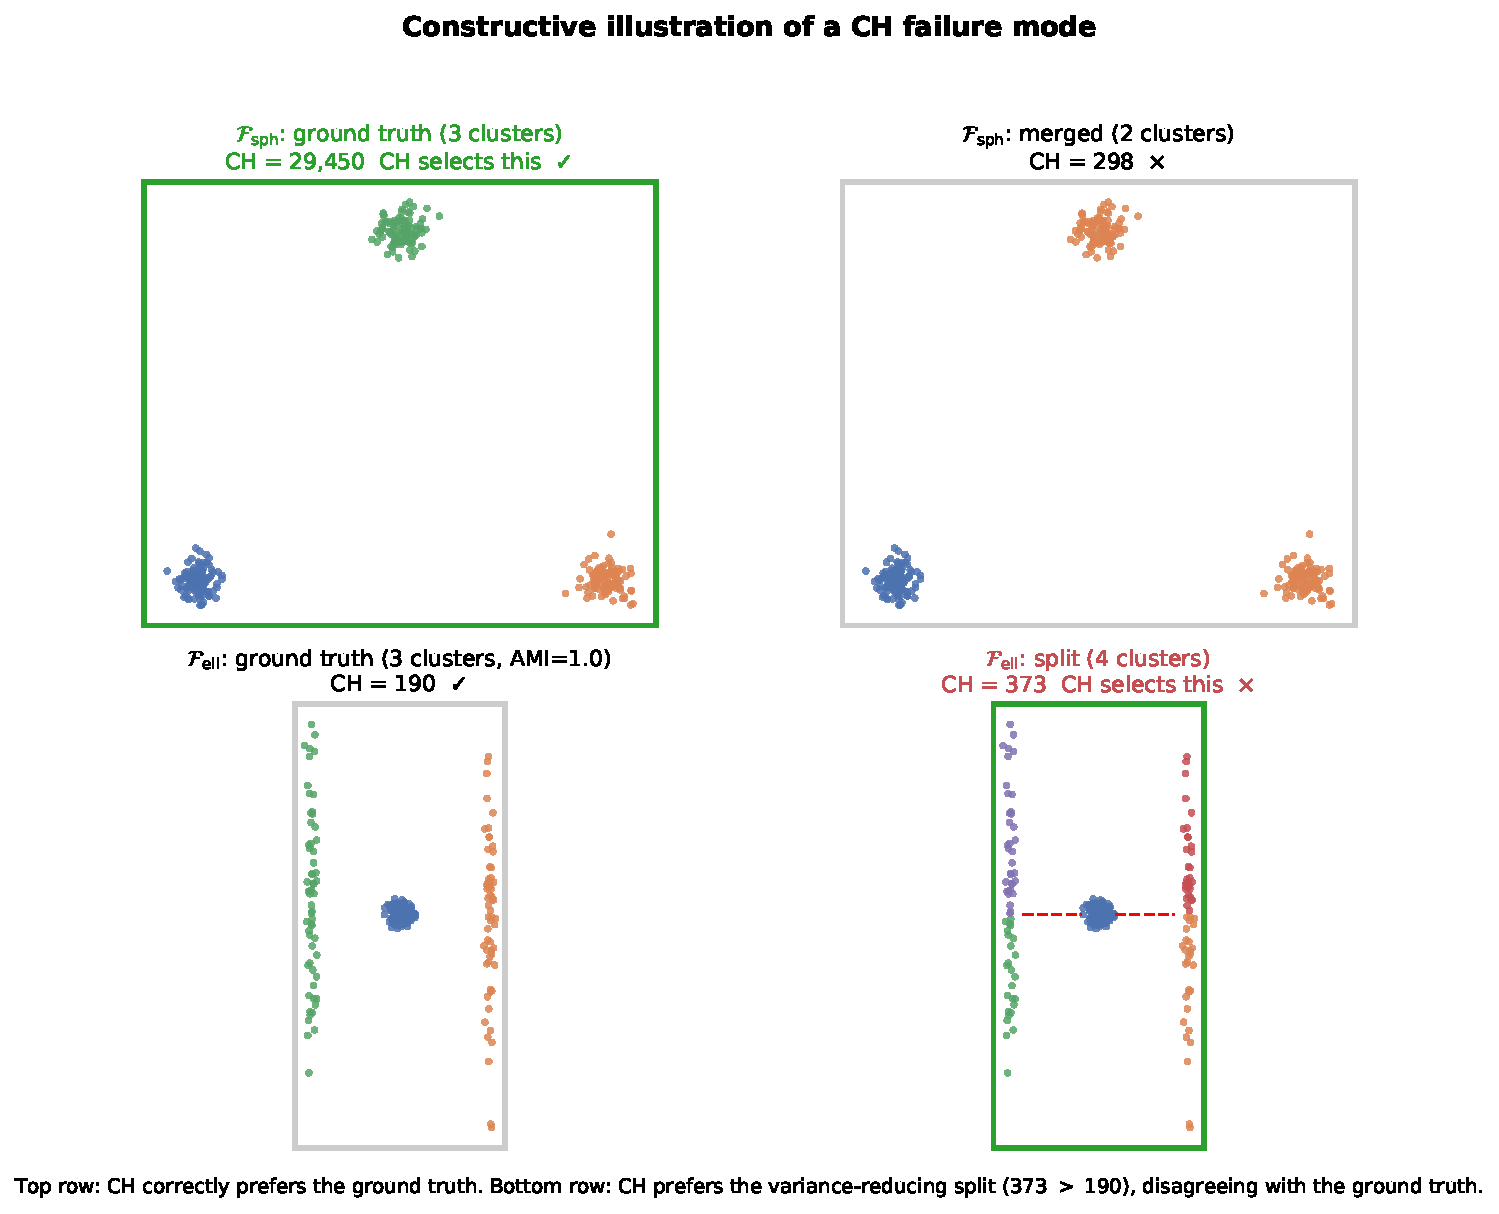
\includegraphics[width=\textwidth]{figure3_impossibility.pdf}
\caption{Constructive CH failure mode; each row shows a dataset family under two candidate partitions, with the CH-selected partition (higher CH) outlined in green. \textbf{Top ($\mathcal{F}_{\text{sph}}$, isotropic Gaussians):} CH correctly prefers the ground-truth 3-cluster partition (CH=29,450) over the merged 2-cluster partition (CH=298). \textbf{Bottom ($\mathcal{F}_{\text{ell}}$, heterogeneous covariance):} CH incorrectly prefers the partition that splits the elongated clusters (CH=373, dashed red lines) over the ground truth (CH=190, AMI=1.0), because splitting reduces within-cluster variance. The failure is that maximizing CH selects the wrong partition in the bottom row.}
\label{fig:impossibility}
\end{figure}

\paragraph{The construction.} We define two dataset families and, on each, a pair of candidate partitions $\pi_a, \pi_b$. Throughout, let
\[
W(\mathcal{X}, \pi) = \frac{1}{n} \sum_{j=1}^{k} \sum_{i: \pi(i)=j} \|x_i - \mu_j\|^2, \quad B(\mathcal{X}, \pi) = \frac{1}{n} \sum_{j=1}^{k} |C_j| \cdot \|\mu_j - \bar{x}\|^2,
\]
with $\mu_j$ the centroid of cluster $j$ and $\bar{x}$ the global mean.

\textbf{Family $\mathcal{F}_{\text{sph}}$.} Let $\mathcal{X}_1 \subset \mathbb{R}^2$ consist of $n = 300$ points drawn from three isotropic Gaussians with $\sigma = 0.3$ and centers $c_1 = (0, 0)$, $c_2 = (10, 0)$, $c_3 = (5, 8.66)$ (equilateral triangle, side length 10). Consider:
\begin{itemize}
    \item $\pi_a$: the correct 3-cluster assignment (each point to its generating center);
    \item $\pi_b$: a 2-cluster assignment that merges clusters 2 and 3.
\end{itemize}
For this dataset the three isotropic Gaussians are well-separated, so $\pi_a$ has lower $W$ and higher $B$ than $\pi_b$. Empirically (Figure~\ref{fig:impossibility} top row, computed with 100 points per Gaussian and $\sigma = 0.3$) $\text{CH}(\mathcal{X}_1, \pi_a) = 29{,}450 > \text{CH}(\mathcal{X}_1, \pi_b) = 298$, which agrees with $\text{AMI}(\pi_a, y^*) > \text{AMI}(\pi_b, y^*)$.

\textbf{Family $\mathcal{F}_{\text{ell}}$.} Let $\mathcal{X}_2 \subset \mathbb{R}^2$ consist of three groups:
\begin{itemize}
    \item Cluster 1: $n_1 = 400$ points from $\mathcal{N}((0,0), 0.2^2 I)$, a dense, compact sphere;
    \item Cluster 2: $n_2 = 100$ points from $\mathcal{N}((3,0), \text{diag}(0.1^2, 2.5^2))$, a vertically elongated ellipsoid;
    \item Cluster 3: $n_3 = 100$ points from $\mathcal{N}((-3,0), \text{diag}(0.1^2, 2.5^2))$, another vertically elongated ellipsoid.
\end{itemize}
Consider:
\begin{itemize}
    \item $\pi_a$: a 4-cluster partition that keeps the dense sphere as one cluster but splits each ellipsoid horizontally at $y=0$;
    \item $\pi_b$: the correct 3-cluster assignment matching the generating distribution.
\end{itemize}
The four-cluster split $\pi_a$ reduces $W$ (each half-ellipsoid is more compact than the full ellipsoid) and increases $B$ (the half-ellipsoid centroids are further apart vertically). Empirically (Figure~\ref{fig:impossibility} bottom row, computed with 200 points in the dense sphere and 60 points in each elongated ellipsoid) $\text{CH}(\mathcal{X}_2, \pi_a) = 373 > \text{CH}(\mathcal{X}_2, \pi_b) = 190$, but $\text{AMI}(\pi_b, y^*) = 1.0 > \text{AMI}(\pi_a, y^*)$. CH prefers the split that reduces variance even though the split violates the underlying generating structure.

\paragraph{What this demonstrates.} On the two constructed families, CH ranks the correct partition first on $\mathcal{F}_{\text{sph}}$ but last on $\mathcal{F}_{\text{ell}}$, and the mismatch is driven by CH's dependence on $B/W$: splitting an elongated cluster along its major axis always reduces $W$ regardless of whether the split is semantically meaningful. This is the specific empirical signal that partition-structural features (elongation of within-cluster covariance, cluster-size imbalance, graph conductance on the $k$NN graph) are designed to capture, and that CH's $B/W$ summary cannot. We do not extend this argument to other fixed IVMs (Davies-Bouldin, Silhouette, DBCV, S\_Dbw depend on per-cluster or density-based quantities not captured by the $B/W$ ratio, and their failure modes are qualitatively different from CH's, though the benchmark results in Table~\ref{tab:main} show that all of them are outperformed by \ours{} in aggregate).

\paragraph{Empirical verification on the benchmark.} On our benchmark (averaged across 5 seeds), CH achieves positive Spearman $\rho$ on 94\% of test datasets but \emph{negative} $\rho$ on 6\%, meaning that on those 6\% CH actively prefers worse partitions in the ordering sense. \ours{} achieves positive $\rho$ on 98\% and negative on only 2\%. The 6\% negative-correlation rate for CH corresponds to real datasets with non-spherical structure or imbalanced cluster sizes, consistent with the failure mode illustrated above.


\section{Compact Feature Set: Selection Protocol}
\label{app:compact}

The 15-feature compact model is constructed as follows:
\begin{enumerate}
    \item For each of the 5 training seeds, train XGBoost on the training fold and extract feature importances (gain-based).
    \item Rank features by importance for each seed.
    \item Select the 15 features that appear in the top-15 for at least 3 out of 5 seeds.
\end{enumerate}

The resulting 15 features are: \texttt{ivm\_calinski\_harabasz}, \texttt{ds\_mean\_of\_kurtosis}, \texttt{graph\_conductance\_min}, \texttt{entropy}, \texttt{ds\_mean\_of\_skewness}, \texttt{ds\_n\_samples}, \texttt{ds\_pairwise\_dist\_std}, \texttt{cluster\_size\_mean}, \texttt{graph\_conductance\_mean}, \texttt{ds\_pairwise\_dist\_mean}, \texttt{between\_cluster\_var}, \texttt{ds\_pairwise\_dist\_median}, \texttt{ivm\_silhouette}, \texttt{ds\_d\_over\_n}, \texttt{noise\_fraction}.

Eight of these features are stable across \emph{all} 5 seeds: \texttt{ivm\_calinski\_harabasz}, \texttt{ds\_mean\_of\_kurtosis}, \texttt{graph\_conductance\_min}, \texttt{entropy}, \texttt{ds\_mean\_of\_skewness}, \texttt{ds\_n\_samples}, \texttt{ds\_pairwise\_dist\_std}, \texttt{cluster\_size\_mean}. Importantly, feature selection is performed exclusively on training folds; test data is never used for selection.


\section{Additional Experimental Tables}
\label{app:additional_tables}

\begin{figure}[h]
\centering
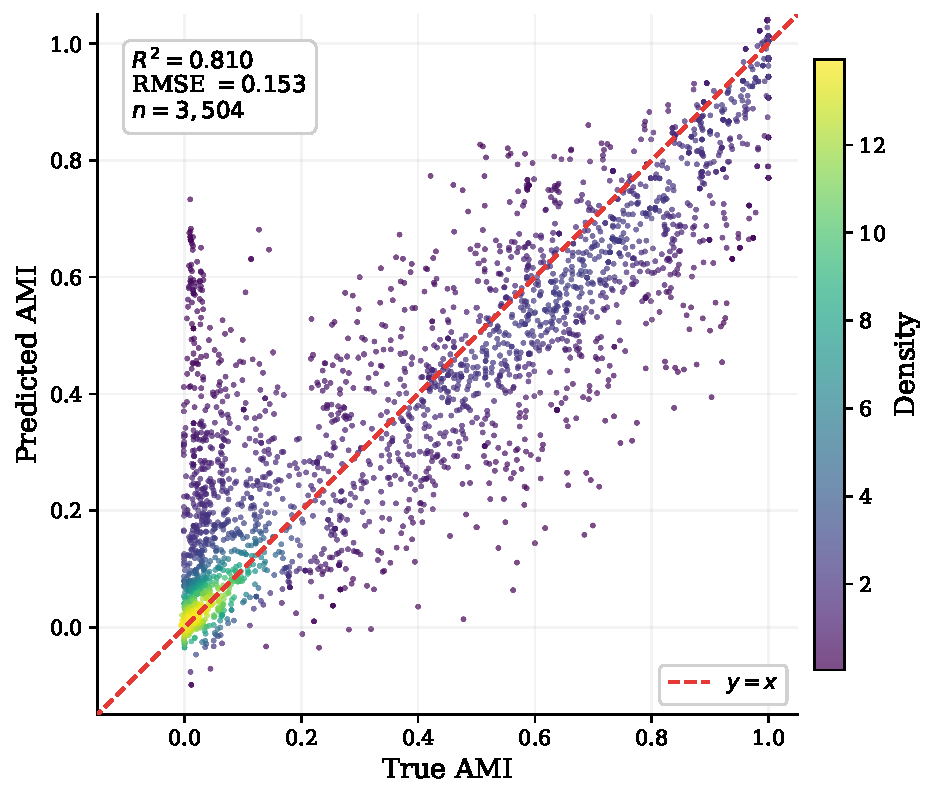
\includegraphics[width=0.6\textwidth]{figure2_scatter.pdf}
\caption{Predicted vs.\ true AMI for all (dataset, partition) pairs on the seed-0 test fold ($R^2 = 0.810$, RMSE $= 0.153$, $n = 3{,}504$: 46 test datasets $\times$ mean 76.2 partitions per dataset). Points near the diagonal indicate accurate prediction. The model captures the full range of external agreement, from poor (AMI $\approx 0$) to excellent (AMI $\approx 1$). Full 5-seed regret and correlation aggregates are in Table~\ref{tab:main} and Table~\ref{tab:correlation}.}
\label{fig:scatter}
\end{figure}

\begin{table}[h]
\centering
\caption{Cross-domain transfer. \ours{} trained on one domain, tested on another. CH shown as reference (the strongest of the three standard compactness-separation IVMs by regret in the in-distribution benchmark).}
\label{tab:transfer}
\small
\begin{tabular}{lcccc}
\toprule
\textbf{Scenario} & \multicolumn{2}{c}{\textbf{\ours{}}} & \multicolumn{2}{c}{\textbf{CH (reference)}} \\
\cmidrule(lr){2-3} \cmidrule(lr){4-5}
& Regret $\downarrow$ & $\rho$ $\uparrow$ & Regret $\downarrow$ & $\rho$ $\uparrow$ \\
\midrule
In-distribution (60/20/20) & $.071$ & $.748$ & $.217$ & $.604$ \\
\midrule
Synthetic $\to$ real & $.100$ & $.678$ & $.235$ & $.489$ \\
Synthetic $\to$ OpenML & $.100$ & $.657$ & $.218$ & $.466$ \\
Synthetic $\to$ image+text & $.105$ & $.887$ & $.398$ & $.722$ \\
\midrule
Real $\to$ synthetic & $.238$ & $.607$ & $.193$ & $.761$ \\
OpenML $\to$ synthetic & $.209$ & $.590$ & $.193$ & $.761$ \\
\bottomrule
\end{tabular}
\end{table}

\begin{table}[h]
\centering
\caption{Leave-one-algorithm-out: impact of removing each algorithm family from training.}
\label{tab:loo}
\small
\begin{tabular}{lcc}
\toprule
\textbf{Held-out Algorithm} & \textbf{Regret (without)} & $\Delta$ \textbf{Regret} \\
\midrule
KMeans & $.047 \pm .084$ & $+.004$ \\
Gaussian Mixture & $.047 \pm .075$ & $+.004$ \\
DBSCAN & $.043 \pm .107$ & $+.023$ \\
HDBSCAN & $.022 \pm .044$ & $-.001$ \\
Agglomerative & $.049 \pm .065$ & $+.004$ \\
\bottomrule
\end{tabular}
\end{table}

\begin{table}[h]
\centering
\caption{Per-dataset Spearman correlation between predicted scores and true AMI (averaged over the 230 seed--dataset test evaluations of the 5-seed 60/20/20 protocol; 158 unique datasets appear in at least one test fold).}
\label{tab:correlation}
\small
\begin{tabular}{lc}
\toprule
\textbf{Method} & \textbf{Spearman} $\rho$ \\
\midrule
\ours{} (predicted) & $\mathbf{0.748 \pm 0.259}$ \\
CH Adjusted \citep{jeon2025measuring} & $0.531 \pm 0.281$ \\
Calinski-Harabasz & $0.604 \pm 0.320$ \\
Silhouette & $0.433 \pm 0.402$ \\
Davies-Bouldin (neg) & $0.399 \pm 0.385$ \\
\bottomrule
\end{tabular}
\end{table}

\begin{table}[h]
\centering
\caption{Preliminary model selection on 7 real-world attributed graphs (189 candidate partitions); regret uses NMI as the external agreement metric. We report a single protocol: 7-fold leave-one-graph-out cross-validation (each fold trains on 6 graphs, tests on the held-out 7th, regret averaged over folds). With only 7 graphs the estimate is high-variance, so we present it as a preliminary indication rather than a headline result. Classical IVMs use only node attributes (Silhouette and CH are anti-correlated with quality); modularity uses only graph structure. Datasets (Cora, CiteSeer, PubMed, Amazon Photo/Computers, Coauthor CS/Physics) are loaded via \texttt{torch\_geometric} and require download.}
\label{tab:attr_graph}
\small
\begin{tabular}{lcc}
\toprule
\textbf{Method} & \textbf{Regret} $\downarrow$ & \textbf{Spearman} $\rho$ $\uparrow$ \\
\midrule
\multicolumn{3}{l}{\textit{Attribute-only baselines (ignore graph structure)}} \\
Silhouette (on node attributes) & $.395$ & $-.588$ \\
Calinski-Harabasz (on node attributes) & $.350$ & $-.481$ \\
Davies-Bouldin (on node attributes) & $.039$ & $.548$ \\
\midrule
\multicolumn{3}{l}{\textit{Graph-only baseline (ignore node attributes)}} \\
Modularity & $.028$ & $.592$ \\
\midrule
\textbf{\ours{} (graph features, 7-fold leave-one-graph-out)} & $\mathbf{.004}$ & $\mathbf{.657}$ \\
\bottomrule
\end{tabular}
\end{table}

\begin{table}[h]
\centering
\caption{Training objective comparison under the paper's exact 5-seed 60/20/20 protocol. All three objectives use the same XGBoost architecture and hyperparameters. Differences are modest relative to the gap over classical IVMs (CH regret $\geq 0.20$).}
\label{tab:ranking_objectives}
\small
\begin{tabular}{lcc}
\toprule
\textbf{Training Objective} & \textbf{Regret} $\downarrow$ & \textbf{Spearman} $\rho$ $\uparrow$ \\
\midrule
Pointwise regression (MSE) & $.068 \pm .012$ & $.761 \pm .033$ \\
LambdaMART (rank:ndcg) & $.062 \pm .017$ & $.782 \pm .021$ \\
Pairwise (rank:pairwise) & $.065 \pm .015$ & $.796 \pm .027$ \\
\midrule
\textit{CH (strongest CS-IVM by $\rho$)} & \textit{.217 $\pm$ .237} & \textit{.604 $\pm$ .320} \\
\bottomrule
\end{tabular}
\end{table}

\begin{table}[h]
\centering
\caption{Selection regret across four external quality metrics (5 seeds, 28-feature set). The AMI regret here (0.076) differs slightly from Table~\ref{tab:main} (0.071) because each metric uses a separately trained model and the averaging scope differs.}
\label{tab:multitarget}
\small
\begin{tabular}{lcccc}
\toprule
\textbf{Method} & \textbf{AMI} & \textbf{ARI} & \textbf{NMI} & \textbf{V-measure} \\
\midrule
\ours{} (XGBoost) & $\mathbf{.076}$ & $\mathbf{.092}$ & $\mathbf{.072}$ & $\mathbf{.072}$ \\
Ridge & $.123$ & $.152$ & $.125$ & $.125$ \\
\midrule
Calinski-Harabasz & $.217$ & $.250$ & $.219$ & $.219$ \\
Silhouette & $.342$ & $.380$ & $.340$ & $.340$ \\
Davies-Bouldin & $.345$ & $.374$ & $.345$ & $.345$ \\
\bottomrule
\end{tabular}
\end{table}

\begin{table}[h]
\centering
\caption{Paired Wilcoxon signed-rank tests: \ours{} (XGBoost) vs.\ each baseline. Per-dataset regret averaged across 5 seeds, 158 test datasets.}
\label{tab:significance}
\small
\begin{tabular}{lcccr}
\toprule
\textbf{Comparison} & \textbf{XGB wins} & \textbf{Baseline wins} & \textbf{Ties} & \textbf{$p$-value} \\
\midrule
vs. Calinski-Harabasz & 110 & 39 & 9 & $4.1 \times 10^{-13}$ \\
vs. Silhouette & 139 & 13 & 6 & $1.5 \times 10^{-24}$ \\
vs. Davies-Bouldin & 137 & 15 & 6 & $2.4 \times 10^{-24}$ \\
vs. Ridge & 74 & 69 & 15 & $2.2 \times 10^{-2}$ \\
\bottomrule
\end{tabular}
\end{table}

\begin{table}[h]
\centering
\caption{Learning curves: regret and Spearman $\rho$ vs.\ training set size (fraction of 133 datasets, 5 seeds).}
\label{tab:learning}
\small
\begin{tabular}{rrccccc}
\toprule
\textbf{Frac.} & $N_{\text{train}}$ & \multicolumn{2}{c}{\textbf{XGBoost}} & \multicolumn{2}{c}{\textbf{Ridge}} \\
\cmidrule(lr){3-4} \cmidrule(lr){5-6}
& & Regret $\downarrow$ & $\rho$ $\uparrow$ & Regret $\downarrow$ & $\rho$ $\uparrow$ \\
\midrule
10\% & 13 & .116 & .717 & .108 & .622 \\
20\% & 26 & .117 & .696 & .108 & .624 \\
30\% & 39 & .085 & .739 & .107 & .625 \\
50\% & 66 & .083 & .758 & .110 & .629 \\
70\% & 93 & .085 & .759 & .126 & .625 \\
100\% & 133 & .076 & .760 & .123 & .634 \\
\bottomrule
\end{tabular}
\end{table}

\begin{table}[h]
\centering
\caption{Top failure cases: datasets with highest average selection regret for \ours{} (XGBoost), across 5 seeds.}
\label{tab:failure}
\small
\begin{tabular}{lrrl}
\toprule
\textbf{Dataset} & \textbf{Regret} & \textbf{Best AMI} & \textbf{Failure mode} \\
\midrule
synth\_uniform\_noise\_2d & 0.658 & 0.989 & High noise, ambiguous structure \\
synth\_subspace\_5of50 & 0.575 & 0.996 & Subspace clustering \\
synth\_imb\_many\_small\_d15 & 0.429 & 1.000 & Extreme imbalance \\
synth\_blobs\_many\_2d & 0.379 & 0.992 & Many clusters, 2D \\
openml\_1040 (sylva\_prior) & 0.367 & 0.478 & High-d (108), low signal \\
synth\_moons\_noise0.15 & 0.327 & 0.818 & Non-convex + noise \\
synth\_mixed\_shapes\_2d & 0.309 & 1.000 & Mixed cluster shapes \\
\bottomrule
\end{tabular}
\end{table}

\begin{table}[h]
\centering
\caption{Asymptotic complexity per dataset with $n$ samples, $d$ features, $k$ clusters, and $M$ candidate partitions. \ours{} is cheaper than Silhouette and comparable to CH/DB.}
\label{tab:complexity}
\small
\begin{tabular}{lll}
\toprule
\textbf{Component} & \textbf{Complexity} & \textbf{Note} \\
\midrule
\multicolumn{3}{l}{\textit{\ours{} (deployment)}} \\
$k$NN graph & $O(n \log n \cdot d)$ & One-time per dataset, reusable \\
Feature extraction & $O(M \cdot n \cdot k)$ & Per partition: cluster stats + graph features \\
Model inference & $O(M \cdot T \cdot d_f)$ & $T{=}$trees, $d_f{=}28$ features; $< 1$\,ms \\
\textbf{Total} & $O(n \log n \cdot d + M \cdot n \cdot k)$ & \\
\midrule
\multicolumn{3}{l}{\textit{Classical IVMs}} \\
Silhouette & $O(M \cdot n^2)$ & Pairwise distance matrix per partition \\
Calinski-Harabasz & $O(M \cdot n \cdot k)$ & Comparable to \ours{} \\
Davies-Bouldin & $O(M \cdot n \cdot k)$ & Comparable to \ours{} \\
\bottomrule
\end{tabular}
\end{table}


\begin{table}[h]
\centering
\caption{Candidate-pool robustness. \ours{} trained on the full pool, tested on modified pools at test time. \ours{} outperforms CH across all 11 configurations, supporting the view that the learned surrogate is not specialized to a particular candidate menu.}
\label{tab:pool_robust}
\small
\begin{tabular}{lcc}
\toprule
\textbf{Pool configuration} & \textbf{\ours{} regret} $\downarrow$ & \textbf{CH regret} \\
\midrule
Full pool (all algorithms) & $.057$ & $.199$ \\
\midrule
Drop KMeans & $.053$ & $.205$ \\
Drop GaussianMixture & $.048$ & $.183$ \\
Drop DBSCAN & $.055$ & $.134$ \\
Drop HDBSCAN & $.059$ & $.191$ \\
Drop AgglomerativeClustering & $.054$ & $.195$ \\
\midrule
KMeans only & $.036$ & $.085$ \\
Density-based only (DBSCAN+HDBSCAN) & $.023$ & $.119$ \\
Random 50\% subsample & $.055$ & $.174$ \\
Only $k \geq 5$ & $.054$ & $.139$ \\
Only $k \leq 3$ & $.042$ & $.127$ \\
\bottomrule
\end{tabular}
\end{table}


\end{document}
